\documentclass{beamer}
\usecolortheme{wolverine}

\setbeamertemplate{caption}{\raggedright\insertcaption\par}

\usepackage{soul}
\usepackage{relsize}
\usepackage{tabularx}
\usepackage{booktabs}
\usepackage{multirow}
\newcolumntype{C}{>{\centering\arraybackslash}X}
\usepackage{proof}
\usepackage{amsmath}
\usepackage{wasysym}
\usepackage{tikz}
\usetikzlibrary{arrows.meta,positioning,matrix, shapes.multipart, calc}
\usepackage{tikz-qtree}
\usepackage{hyperref}
\hypersetup{
    colorlinks=true,
    linkcolor=blue,
    filecolor=magenta,      
    urlcolor=blue,
}
\newcommand{\posimpl}{\overset{+}{\multimap}}
\newcommand{\negimpl}{\overset{-}{\multimap}}
\newcommand{\posat}[1]{\overset{+}{\proofspace#1}}
\newcommand{\negat}[1]{\overset{-}{\proofspace#1}}
\newcommand{\proofspace}{\vphantom{()}}

\newcommand{\term}[1]{\ensuremath{\mathtt{#1}}}
\newcommand{\li}{\!\multimap\!}
\newcommand{\lotimes}{\!\otimes\!}
\newcommand{\loplus}{\!\oplus\!}
\newcommand{\lin}[1]{\langle#1\rangle}
\newcommand{\lint}[1]{[#1]}
\newcommand{\cat}[1]{\footnotesize \textsc{#1}}	
\newcommand{\W}[1]{\scriptsize #1}
\newcommand{\etext}[1]{\scriptsize {\textit{#1}}}
\newcommand{\smain}{\cat{S}$_{\text{main}}$}
\newcommand{\ssub}{\cat{S}$_{\text{sub}}$}
\newcommand{\type}[2]{\scriptsize\ensuremath{\textcolor{#2}{#1}}}
\newcommand{\red}[1]{\textcolor{red}{{}_#1}}
\newcommand{\redat}[2]{\alt<{#1}>{\textcolor{red}{#2}}{#2}}
\newcommand{\dia}{\ensuremath{\diamondsuit}}
\newcommand{\dx}[1]{\overset{#1}{\dia}}
\newcommand{\bx}[1]{\overset{#1}{\Box}}


\usetikzlibrary{matrix, arrows.meta, calc, positioning, arrows}

\title{Type \& Proof Extraction}
\author{Kokos}
\institute{Logic \& Language \st{2020}2021\footnote{\smaller totally not the same slides as last year}}
\date{16/12/21}

\begin{document}


\title{Data-driven Logic}
\subtitle{or: type theory for the working engineer}

\maketitle

\begin{frame}{The state of NLP affairs}
	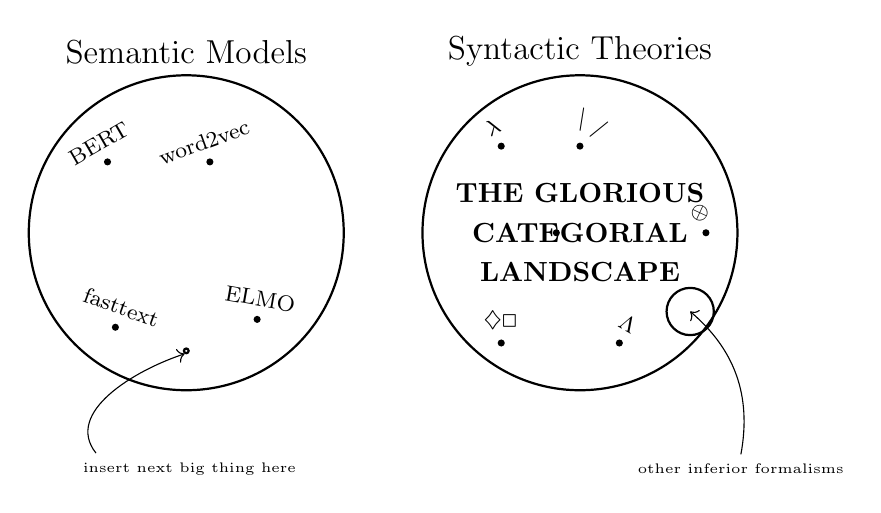
\begin{tikzpicture}
		[elem/.style = {circle, thick, draw, solid, opacity=1, inner sep=.75\pgflinewidth}, fill=black]
		\node (sems) at (0, 2.3) {\larger{Semantic Models}};
		\draw[thick] (0,0) circle (2cm);
			\node[label={[rotate=30]\smaller BERT},elem,fill=black] (bert) at (-1, 0.9) {};
			\node[label={[rotate=-10]\smaller ELMO},elem,fill=black] (elmo) at (0.9, -1.1) {};
			\node[label={[rotate=20]\smaller word2vec},elem,fill=black] (w2v) at (0.3, 0.9) {};
			\node[label={[rotate=-20]\smaller fasttext},elem,fill=black] (ft) at (-0.9, -1.2) {};
			\node[elem] (A) at (0, -1.5) {};
			\node (B) at (0, -3) {\smaller[3] insert next big thing here};
			\draw[->, bend left, out=80] (B) to (A);
		\draw[thick] (5,0) circle (2cm);
		\node (syn) at (5, 2.3) {\larger Syntactic Theories};
			\visible<2->{
				\node (tg) at (5, 0.5) {\textbf{THE GLORIOUS}};
				\node (tg2) at (5,0) {\textbf{CATEGORIAL}};
				\node (tg3) at (5, -0.5) {\textbf{LANDSCAPE}};
				\visible<3->{
					\draw[thick] (6.4, -1) circle (0.3cm);
					\node (C) at (7, -3) {\smaller[3] other inferior formalisms};
					\draw[->, bend right] (C) to (6.4, -1);
				}			
			}
			\node[label={[rotate=30]\smaller $\lambda$},elem,fill=black] (l) at (4, 1.1) {};
			\node[label={[rotate=-30]\smaller $\Lambda$},elem,fill=black] (l) at (5.5, -1.4) {};
			\node[label={[rotate=0]\smaller $\dia\Box$},elem,fill=black] (l) at (4, -1.4) {};
			\node[label={[rotate=20]\smaller $\li$},elem,fill=black] (l) at (4.7, 0) {};
			\node[label={[rotate=-30]\smaller $\backslash$ /},elem,fill=black] (l) at (5, 1.1) {};
			\node[label={[rotate=--20]\smaller $\otimes$},elem,fill=black] (l) at (6.6, 0) {};
	\end{tikzpicture}
	
	\visible<4->
{	\begin{block}{What's missing?}
		\visible<5->{No (working) unifying theory or application.}
	\end{block}
}
\end{frame}


\begin{frame}{Neural Type-Driven Representations}
\small
The agenda:
\begin{itemize}
	\item[$\lambda$] \alt<2->{\alert{Choosing the logic}}{Choosing the logic}
	\item[$\lambda$] \alt<2->{\alert{Making a dataset: proofs and lexical type assignments}}{Making a dataset: proofs and lexical type assignments}
	\item[$\lambda$] \alt<2->{\textcolor{gray}{Learning the type assignment process}}{Learning the type assignment process}
	\item[$\lambda$] \alt<2->{\textcolor{gray}{Navigating the proof space}}{Navigating the proof space}
	\item[$\lambda$] \alt<2->{\textcolor{gray}{Syntax-aware \& type-correct text representations}}{Syntax-aware \& type-correct text representations}
\end{itemize}
\end{frame}

\begin{frame}{\alt<3->{A twist}{Syntax-Semantics Interface}}
%	 tlg : syntax -> der -> sem
%	 acg: 	tecto	-> pheno
%					-> sem
%	 now:	pheno	-> syntax	-> der	-> sem
%	 		we leave the pointwise translation from pheno to syntax implicit, avoiding the trap of ACG exploding lexicon
%			parse instead directly on tectogrammatic form
%			the lambda terms obtained are the same as doing pheno -> tecto (.) parse (.) tecto-> pheno 

	\alt<3->{
		\centering
		Now
		\vspace{5pt}
		
		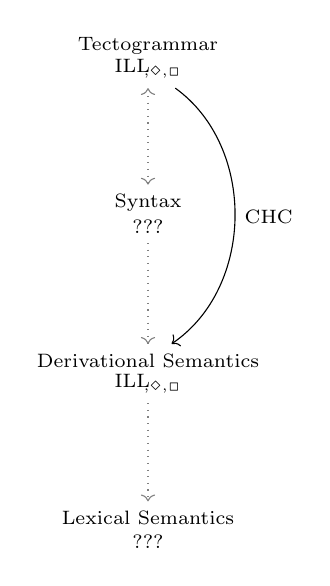
\begin{tikzpicture}
			\node (abstract)	at	(0, 0) 		{\scriptsize Tectogrammar};
			\node (depill)	at	(0, -0.3)	{\scriptsize ILL$_{\li, \Diamond, \Box}$};
			\node (syntax)	at 	(0, -2)		{\scriptsize Syntax};
			\node (depnl)	at 	(0,	-2.3)	{\scriptsize ???};
			\node (der)		at	(0, -4)		{\scriptsize Derivational Semantics};
			\node (derill)	at 	(0, -4.3)	{\scriptsize ILL$_{\li, \Diamond, \Box}$};
			\node (sem)		at 	(0, -6)		{\scriptsize Lexical Semantics};
			\node (seml)		at	(0, -6.3)	{\scriptsize ???}; 
			
			\draw (depill) edge[bend left=55, ->] node[right] {\scriptsize CHC} (der);
			\draw (depill) 	edge[<->, gray, dotted] (syntax);
			\draw (depnl)	edge[->, gray, dotted] (der); 
			\draw (derill) 	edge[->, gray, dotted] (sem);
		\end{tikzpicture}
	}{
		\begin{minipage}[t]{0.5\textwidth}
			\centering Type-logical perspective
			\vspace{5pt}
			
			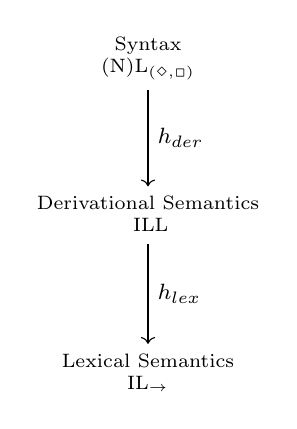
\begin{tikzpicture}
				\node (syntax) at (0,0) {\scriptsize Syntax};	
				\node (nl) at (0,-0.3) {\scriptsize (N)L$_{(\Diamond, \Box)}$};
				\node (der) at (0,-2) {\scriptsize Derivational Semantics};
				\node (mill) at (0,-2.3) {\scriptsize ILL$_{\li}$};
				\node (sem) at (0,-4) {\scriptsize Lexical Semantics};
				\node (il) at (0, -4.3) {\scriptsize IL$_{\to}$};
		
				\draw (nl) edge[->] node[midway, right] {\footnotesize $h_{der}$} (der);
				\draw (mill) edge[->] node[midway, right] {\footnotesize $h_{lex}$} (sem);
			\end{tikzpicture}		
			\end{minipage}%
			\pause
			\begin{minipage}[t]{0.5\textwidth}
					\centering ACG perspective
					\vspace{5pt}
					
			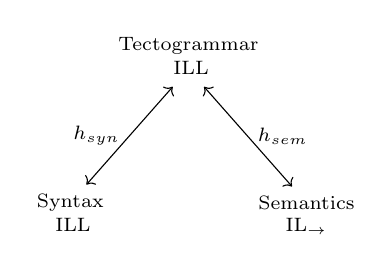
\begin{tikzpicture}		
				\node (abstract) 	at 	(0, 0) 		{\scriptsize Tectogrammar};
				\node (amill)		at	(0, -0.3)	{\scriptsize ILL$_{\li}$};
				\node (syntax)		at	(-1.5, -2) 	{\scriptsize Syntax};
				\node (symill) 		at	(-1.5, -2.3)	{\scriptsize ILL$_{\li}$};
				\node (semantics)	at 	(1.5, -2) 	{\scriptsize Semantics};
				\node (semill)		at	(1.5, -2.3)	{\scriptsize IL$_{\to}$};
				\draw (amill) edge[<->] node[midway, left] {\scriptsize $h_{syn}$} (syntax);
				\draw (amill) edge[<->] node[midway, right] {\scriptsize $h_{sem}$} (semantics);
			\end{tikzpicture}		
		\end{minipage}
	}
\end{frame}

\begin{frame}{Abstract syntax with NLP}
\small
\alt<2->{
	Lexicon $\mathcal{L}$ assigning words types from: $\visible<3->{A \ 
							\visible<4->{ | \ \Diamond^d T \li T' \ 
							\visible<5->{ | \ \Box^d \left( T \li T'\right) }}}$
	
	\vfill

	\begin{minipage}[t]{0.9\textwidth}
		\begin{tabularx}{0.9\textwidth}{rlcrl}
		\visible<3->{animals, ducks, I & : $np$} & & \visible<4->{fly, swim & : $\Diamond^{su}np \li s$}\\
		\visible<4->{like & : $\Diamond^{obj}np \li \Diamond^{obj}np \li s$} & & \visible<5->{gracefully & : $\Box^{mod}\left(s \li s \right)$}\\
		\visible<6->{that & \multicolumn{4}{l}{: $\Diamond^{body}\left(\Diamond^{su} np \li s\right) \li \Box^{mod}\left(np\li np \right)$}}\\
		\end{tabularx}
	\end{minipage}		

	\begin{minipage}{0.99\textwidth}		
		\scriptsize
		\centering
		\alt<3>{
			\[
				\infer[\mathcal{L}]{\term{ducks}: np}{\text{ducks}}
			\]}
		{
		\alt<4>{
			\[
				\infer[\li E]{\langle \text{ducks} \rangle^{su} \  \text{fly} \vdash  s}{
					\infer[\mathcal{L}]{\Diamond^{su}np \li s}{\text{fly}}
					&
					\infer[\Diamond^{su} I]{\langle \text{ducks} \rangle^{su} \vdash \Diamond^{su} np}{
						\infer[\mathcal{L}]{np}{\text{ducks}}
					}
				}
			\]
			\[
				\term{fly} \ \vartriangle^{su}\term{ducks}
			\]
		}{
		\alt<5>{
			\[
				\infer[\li E]{\langle \text{ducks} \rangle^{su} \ \text{fly} \ \langle \text{gracefully} \rangle^{mod} 
				\vdash  s}{
					\infer[\Box^{mod} E]{\langle \text{gracefully} \rangle^{mod} \vdash s \li s }{
						\infer[\mathcal{L}]{\Box^{mod} \left( s \li s \right)}{\text{gracefully}}
					}
					&
					\infer{\langle \text{ducks} \rangle^{su} \  \text{fly} \vdash s}{
						\infer*{}{}
					}
				}
			\]
			\[
				\blacktriangledown^{mod}\term{gracefully} \ (\term{fly} \ \vartriangle^{su}\term{ducks})
			\]
		}{
		\alt<6>{
			\scriptsize
			\[
				\hspace{-5pt}
				\infer[\li E]{\text{animals}\ \langle \text{that}\ \langle \langle\text{I}\rangle^{su}~\text{like}\rangle^{body}\rangle^{mod} \vdash np}{
					\infer[\mathcal{L}]{np}{\text{animals}}
					&
					\hspace{-40pt}
					\infer[\Box^{mod} E]{\langle \text{that}\ \langle \langle\text{I}\rangle^{su}~\text{like}\rangle^{body}\rangle^{mod}\vdash np \li np}{
						\infer[\li E]{\text{that}\ \langle \langle\text{I}\rangle^{su}~\text{like}\rangle^{body} \vdash \Box^{mod} (np \li np)}{
							\infer[\mathcal{L}]{\Diamond^{body}\left(\Diamond^{obj} np \li s\right) \li \Box^{mod}\left(np\li np \right)}{\text{that}}
							&
							\infer[\Diamond^{body} I]{\langle \langle\text{I}\rangle^{su}~\text{like}\rangle^{body} \vdash \Diamond^{body}\left(\Diamond^{obj} np \li s \right)}{
								\infer*[]{\langle\text{I}\rangle^{su}~\text{like} \vdash \lambda x.(\term{like}~x~\vartriangle^{su}\!\!I): \Diamond^{obj}np\li s}{}
							}
						}
					}
				}
			\]
			\[
				\blacktriangledown^{mod}\left(\term{that} \ \vartriangle^{body}\left(\!\lambda x.(\term{like}\ \term{x}\ \vartriangle^{su}\!\!I)\right)\right)~\term{animals}
			\]
		}}}}{}
	\end{minipage}

	
}{
	\begin{block}{Grammar}
		ILL$_{\li}$ plus $\Diamond, \Box$ modalities for \textit{dependency domain demarkation}.
	\end{block}
	\vfill
		
	Types inductively defined by:
	\[
		\mathcal{T} := A \ | \  T \li T' \ | \ \Diamond^d  T \ | \ \Box^d T \qquad A \in \mathcal{A}, T \in \mathcal{T}
	\]
	\vfill	

	\begin{block}{Rules}
	\begin{align*}
		\infer[\li E]{\Gamma, \Delta \vdash \term{s\ t}: B}{\Gamma \vdash \term{s}: A \li B & \Delta \vdash \term{t}: A}
		&\qquad
		\infer[\li I]{\Gamma \vdash \term{\lambda x.s}: A \li B}{\Gamma, \term{x}: A \vdash \term{s}: B} \\
		\infer[\Diamond^d I]{\langle \Gamma \rangle^{d} \vdash \vartriangle^d \term{t}: \Diamond^d A}{\Gamma \vdash \term{t}: A}
		&\qquad
		\infer[\Diamond^d E]{X[Y] \vdash \term{t}[\triangledown^d \term{s}/\term{x}]: B}{
			Y \vdash \term{s}: \Diamond^d A
			&
			X[\langle \term{x}: A \rangle^d] \vdash \term{t}: B} \\
		\infer[\Box^d I]{X \vdash \blacktriangle^d \term{s}: \Box^d A}{\langle X \rangle^d \vdash \term{s}: A}
		&
		\qquad
		\infer[\Box^d E]{\langle X \rangle^d \vdash \blacktriangledown^d \term{s}: A}{X \vdash \term{s}: \Box^d A}
	\end{align*}
	\end{block}
}
\end{frame}

\begin{frame}{Why ILL$_{\li, \Diamond, \Box}$?}
\small
\begin{block}{Why ILL$_{\li}$?}
	\begin{itemize}
	\item Easier to extract from corpora
	\item Massive reduction in lexical ambiguity (more later)
	\item Abstract away from trivial word-order permutations
	\item Surface syntax matters little to semantics
	\end{itemize}
\end{block}

\pause
\begin{block}{Why $\Diamond, \raisebox{1.5pt}{\ensuremath{\Box}}$?}
	\begin{itemize}
	\item More interpretation options
	\item Subsume dependency parsing
	\item More informative for semantics 
	\item Modalities can regulate non-logical parsing
	\end{itemize}
\end{block}
\end{frame}

\begin{frame}{Intermezzo: Proof Nets}
	
	\alt<13->{
			\smaller
			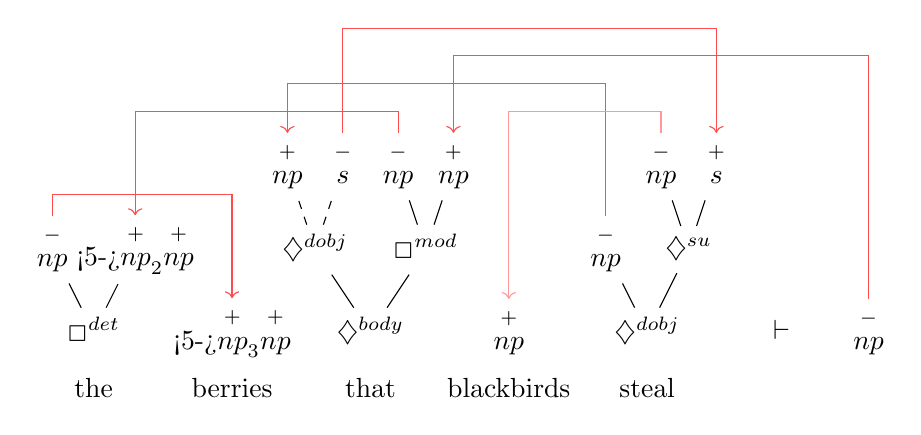
\begin{tikzpicture}
		
%		% words
			\node (the)		at 	(0em, 0em)	{the};
			\node (berries)	at 	(5em, 0em)	{berries};
			\node (that)		at 	(10em, 0em)	{that};
			\node (birds) 	at 	(15em, 0em) 	{blackbirds};
			\node (steal)	at	(20em, 0em)	{steal};
			
%			\visible<3->{
			% undecorated trees
			\node (thedet)		at	(0em, 2em)		{$\Box^{det}\proofspace$};
			\node (thenp1)		at	(-1.5em, 5em)	{$\negat{np}$};
			\node (thenp2)		at	(1.5em, 5em)		
				{\alt<5->{$\posat{np}_2$}{$\posat{np}$}};
			\node (berriesnp)	at 	(5em, 2em)		
				{\alt<5->{$\posat{np}_3$}{$\posat{np}$}};
			\node (thatbody)		at	(10em, 2em)		{$\diamondsuit^{body}\proofspace$};
			\node (thatobj)		at	(8em, 5em)		{$\diamondsuit^{dobj}\proofspace$};
			\node (thatobjnp)	at	(7em, 8em)		{$\posat{np}$};
			\node (thats)		at	(9em, 8em)		{$\negat{s}$};
			\node (thatmod)		at	(12em, 5em)		{$\Box^{mod}\proofspace$};
			\node (thatmodnp1)	at	(11em, 8em)		{$\negat{np}$};
			\node (thatmodnp2)	at	(13em, 8em)		{$\posat{np}$};
			\node (birdsnp)		at	(15em, 2em)		{$\posat{np}$};
			\node (stealobj)		at	(20em, 2em)		{$\diamondsuit^{dobj}\proofspace$};
			\node (stealobjnp)	at	(18.5em, 5em)	{$\negat{np}$};
			\node (stealsu)		at	(21.5em, 5em)	{$\diamondsuit^{su}\proofspace$};
			\node (stealsunp)	at  (20.5em, 8em)	{$\negat{np}$};
			\node (steals)		at 	(22.5em, 8em)	{$\posat{s}$};
			\node (vdash)		at 	(25em, 2em)		{$\vdash\proofspace$};
			\node (finalnp)		at 	(28em, 2em)		{$\negat{np}$};
			
			% internal links
			\draw (thedet)   -- (thenp1);
			\draw (thedet)   -- (thenp2);
			\draw (stealobj) -- (stealobjnp);
			\draw (stealobj) -- (stealsu);
			\draw (stealsu)  -- (stealsunp);
			\draw (stealsu)  -- (steals);
			\draw (thatbody) -- (thatobj);
			\draw (thatobj)   edge[dashed] (thatobjnp);
			\draw (thatobj)   edge[dashed] (thats);
			\draw (thatmod)  -- (thatmodnp1);
			\draw (thatmod)  -- (thatmodnp2);
			\draw (thatbody) -- (thatmod);
			
			% axiom links
			\visible<9->{
			\draw[<-, red!70] (berriesnp) -- ($(berriesnp) + (0em, 5em)$) -| (thenp1);
			\draw[<-, red!70] (thenp2) -- ($(thenp2) + (0em, 5em)$) -| (thatmodnp1);
			\draw[<-, red!70] (thatobjnp) -- ($(thatobjnp) + (0em,3em)$) -| (stealobjnp);
			\draw[->, red!70] (thats) -- ($(thats) + (0em, 5em)$) -| (steals);
			\draw[<-, red!70] (thatmodnp2) -- ($(thatmodnp2) + (0em, 4em)$) -| (finalnp);
			\draw[<-, red!40] (birdsnp) -- ($(birdsnp) + (0em, 8em)$) -| (stealsunp);
			}
		\end{tikzpicture}
	}{
	\alt<12>{
	\begin{block}{Traversing a Proof Net}
	\smaller[2]
	\textbf{positive (down) mode}: start from positive leaf, follow positive nodes to subtree root
	\begin{itemize}
		\item[$\Box$] wrap future with $\blacktriangledown$ 
		\item[$\dia$] wrap variable (context) with $\triangledown$
		\item[$\li$] each is an application\\
		on reaching root, write word or variable name\\
		and perform negative traversal on negative child of each $\li$
	\end{itemize}
	\textbf{	negative (up) mode}: start from negative root, follow negatives to subtree leaf
	\begin{itemize}
		\item[$\Box$] wrap future with $\blacktriangle$
		\item[$\dia$] wrap future with $\vartriangle$
		\item[$\li$] each is an abstraction: assign a fresh variable to positive subtree \\
		on reaching a leaf, cross the axiom link and switch to positive mode
	\end{itemize}
		
	
	start from conclusion in negative mode
	\end{block}
	}
	{
	\alt<10->{
		\begin{block}{\alt<11->{Proof Structure}{Proof Frame}}
		{\smaller
		\alt<11->{A proof net together with \textbf{axiom links}: bijection between pos/neg atoms}{A sequence of polarized unfolded formulas}}
		\vspace{10pt}

		\smaller
		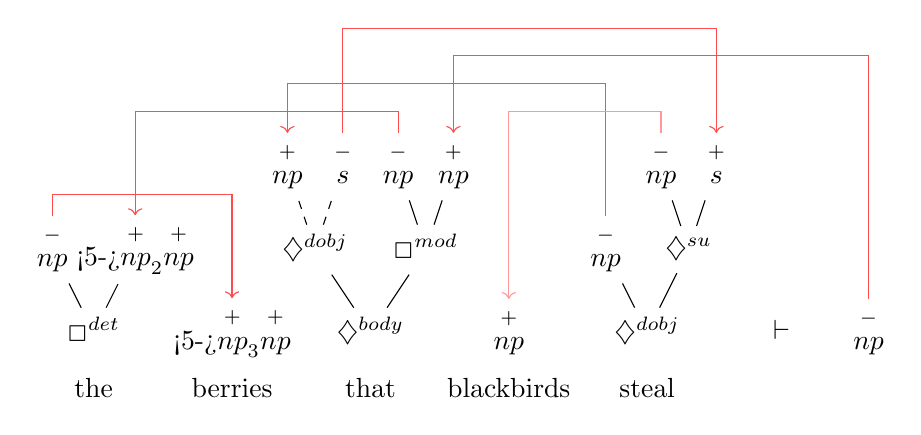
\begin{tikzpicture}
		
%		% words
			\node (the)		at 	(0em, 0em)	{the};
			\node (berries)	at 	(5em, 0em)	{berries};
			\node (that)		at 	(10em, 0em)	{that};
			\node (birds) 	at 	(15em, 0em) 	{blackbirds};
			\node (steal)	at	(20em, 0em)	{steal};
			
%			\visible<2-2>{
%			\draw[->] (that) -- ($(10em, 4em)$);
%			\node (test) 	at 	(10em, 5em) {
%			$\Box^{det}, np, np, \#, np, \#, \diamondsuit^{body}, \diamondsuit^{dobj}, np, s, \Box^{mod}, np, np, \#, \diamondsuit^{dobj}, np, \diamondsuit^{su}, np, s$
%			};
%			}
%			\visible<3->{
			% undecorated trees
			\node (thedet)		at	(0em, 2em)		{$\Box^{det}\proofspace$};
			\node (thenp1)		at	(-1.5em, 5em)	{$\negat{np}$};
			\node (thenp2)		at	(1.5em, 5em)		
				{\alt<5->{$\posat{np}_2$}{$\posat{np}$}};
			\node (berriesnp)	at 	(5em, 2em)		
				{\alt<5->{$\posat{np}_3$}{$\posat{np}$}};
			\node (thatbody)		at	(10em, 2em)		{$\diamondsuit^{body}\proofspace$};
			\node (thatobj)		at	(8em, 5em)		{$\diamondsuit^{dobj}\proofspace$};
			\node (thatobjnp)	at	(7em, 8em)		{$\posat{np}$};
			\node (thats)		at	(9em, 8em)		{$\negat{s}$};
			\node (thatmod)		at	(12em, 5em)		{$\Box^{mod}\proofspace$};
			\node (thatmodnp1)	at	(11em, 8em)		{$\negat{np}$};
			\node (thatmodnp2)	at	(13em, 8em)		{$\posat{np}$};
			\node (birdsnp)		at	(15em, 2em)		{$\posat{np}$};
			\node (stealobj)		at	(20em, 2em)		{$\diamondsuit^{dobj}\proofspace$};
			\node (stealobjnp)	at	(18.5em, 5em)	{$\negat{np}$};
			\node (stealsu)		at	(21.5em, 5em)	{$\diamondsuit^{su}\proofspace$};
			\node (stealsunp)	at  (20.5em, 8em)	{$\negat{np}$};
			\node (steals)		at 	(22.5em, 8em)	{$\posat{s}$};
			\node (vdash)		at 	(25em, 2em)		{$\vdash\proofspace$};
			\node (finalnp)		at 	(28em, 2em)		{$\negat{np}$};
			
			% internal links
			\draw (thedet)   -- (thenp1);
			\draw (thedet)   -- (thenp2);
			\draw (stealobj) -- (stealobjnp);
			\draw (stealobj) -- (stealsu);
			\draw (stealsu)  -- (stealsunp);
			\draw (stealsu)  -- (steals);
			\draw (thatbody) -- (thatobj);
			\draw (thatobj)   edge[dashed] (thatobjnp);
			\draw (thatobj)   edge[dashed] (thats);
			\draw (thatmod)  -- (thatmodnp1);
			\draw (thatmod)  -- (thatmodnp2);
			\draw (thatbody) -- (thatmod);
			
			% axiom links
			\visible<11->{
			\draw[<-, red!70] (berriesnp) -- ($(berriesnp) + (0em, 5em)$) -| (thenp1);
			\draw[<-, red!70] (thenp2) -- ($(thenp2) + (0em, 5em)$) -| (thatmodnp1);
			\draw[<-, red!70] (thatobjnp) -- ($(thatobjnp) + (0em,3em)$) -| (stealobjnp);
			\draw[->, red!70] (thats) -- ($(thats) + (0em, 5em)$) -| (steals);
			\draw[<-, red!70] (thatmodnp2) -- ($(thatmodnp2) + (0em, 4em)$) -| (finalnp);
			\draw[<-, red!40] (birdsnp) -- ($(birdsnp) + (0em, 8em)$) -| (stealsunp);
			}
		\end{tikzpicture}		
		
		\end{block}
	}{
	\alt<4->{
		\begin{block}{Tree Polarization}
		Let $+$ stand for resources we \textit{have}, $-$ for ones we seek:\\
		\quad		{\smaller $\li$ is polarity preserving for the result, reversing for the argument}
		\vspace{10pt}
		
		\smaller
		\centering
		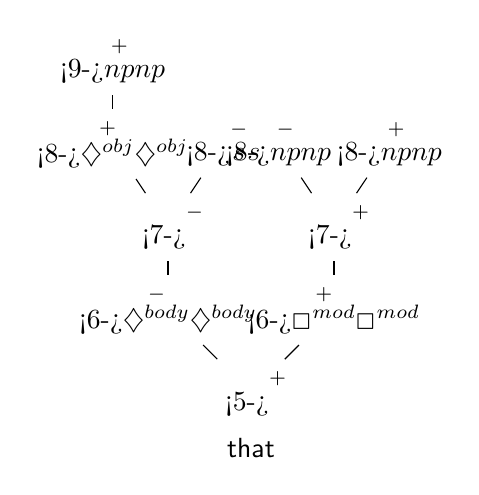
\begin{tikzpicture}		
			\node (that)			at	(10em, 0em)		{$\mathsf{that}$};
			\node (root)			at 	(10em, 2em)		{\alt<5->{$\posat{\li}\proofspace$}{$\li\proofspace$}};
			\node (thatbody)		at 	(7em, 5em)		{\alt<6->{$\negat{\diamondsuit^{body}\proofspace}$}{$\diamondsuit^{body}\proofspace$}};
			\node (thatmod)		at	(13em, 5em)		{\alt<6->{$\posat{\Box^{mod}}\proofspace$}{$\Box^{mod}\proofspace$}};
			\node (right)		at	(13em, 8em)		{\alt<7->{$\posat{\li}\proofspace$}{$\li\proofspace$}};
			\node (left)			at 	(7em, 8em)		{\alt<7->{$\negat{\li}\proofspace$}{$\li\proofspace$}};
			\node (thatobj)		at	(5em, 11em)		{\alt<8->{$\posat{\diamondsuit^{obj}\proofspace}$}{$\diamondsuit^{obj}\proofspace$}};
			\node (thatobjnp)	at	(5em, 14em)		{\alt<9->{$\posat{np\proofspace}$}{$np\proofspace$}};
			\node (thats)		at	(9em, 11em)		{\alt<8->{$\negat{s\proofspace}$}{$s\proofspace$}};
			\node (thatmodnp1)	at	(11em, 11em)		{\alt<8->{$\negat{np\proofspace}$}{$np\proofspace$}};
			\node (thatmodnp2)	at	(15em, 11em)		{\alt<8->{$\posat{np\proofspace}$}{$np\proofspace$}};
			\draw (root) -- (thatbody);
			\draw (root) -- (thatmod);
			\draw (thatbody) -- (left);
			\draw (left) -- (thatobj);
			\draw (thatobj) -- (thatobjnp);
			\draw (left) -- (thats);
			\draw (thatmod) -- (right);
			\draw (right) -- (thatmodnp1);
			\draw (right) -- (thatmodnp2);
%			\draw (thatbody) -- (thatobj);
%			\draw (thatobj)  edge[dashed] (thatobjnp);
%			\draw (thatobj)  edge[dashed] (thats);
%			\draw (thatmod)  -- (thatmodnp1);
%			\draw (thatmod)  -- (thatmodnp2);
%			\draw (thatbody) -- (thatmod);
		\end{tikzpicture}
		\end{block}	
	}{
	\alt<2->{
		\begin{block}{Formula decomposition}
			Type formation rules $\equiv$ tree constructors			
			\vspace{10pt}
		
			\centering
			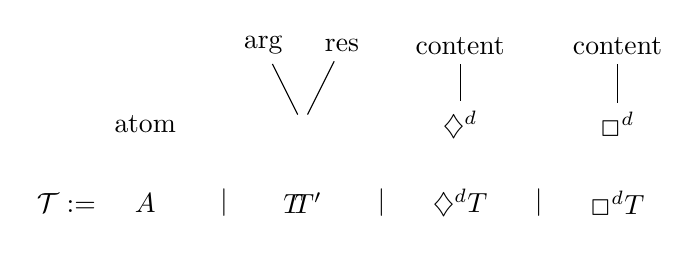
\begin{tikzpicture}
				\node (T) at (-1, -1) {$\mathcal{T}:=$};
				\node (A) at (0, -1) {$A$};
				\node (FN) at (2, -1) {$	T \li T'$};
				\node (DIA) at (4, -1) {$\dia^d T$};
				\node (BOX) at (6, -1) {$\Box^d T$};
				\node (|) at (1, -1) {$|$};
				\node (|) at (3, -1) {$|$};
				\node (|) at (5, -1) {$|$};
				\node (atom) at (0,0) {atom};
				\node (function) at (2, 0) {$\li$};
				\node (left) at (1.5, 1) {arg};
				\node (right) at (2.5, 1) {res};
				\draw (function) -- (left);
				\draw (function) -- (right);
				\node (dia) at (4, 0) {$\dia^d$};
				\node (diac) at (4, 1) {content};
				\draw (dia) -- (diac);
				\node (box) at (6, 0) {$\Box^d$};
				\node (boxc) at (6, 1) {content};
				\draw (box) -- (boxc);
			\end{tikzpicture}
			\visible<3->{
				{\flushright			\smaller{or, overloading $\dia$ and $\Box$ as binary operators for brevity}}
			\vspace{10pt}
			
			\smaller
			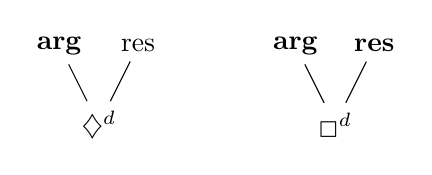
\begin{tikzpicture}
				\node (function) at (2, 0) {$\dia^d$};
				\node (left) at (1.5, 1) {\textbf{arg}};
				\node (right) at (2.5, 1) {res};
				\draw (function) -- (left);
				\draw (function) -- (right);
				\node (function) at (5, 0) {$\Box^d$};
				\node (left) at (4.5, 1) {\textbf{arg}};
				\node (right) at (5.5, 1) {\textbf{res}};
				\draw (function) -- (left);
				\draw (function) -- (right);
			\end{tikzpicture}
			}
		\end{block}
	
	}{
	\begin{block}{Proof Nets}
		\smaller A graphical, diagrammatical representation of (intuitionitic) linear logic proofs.
	\end{block}
	}}}}}
	
\end{frame}

\begin{frame}{From parse graphs to ILL$_{\li, \Diamond, \Box}$ types}
	\small
	\begin{block}{algorithm: graph flooding on dags}
		init with maps
		\begin{itemize}
			\item[-] from pos \& phrasal categories to $\mathcal{A}$	\\
			\quad e.g. $\textsc{np} \to np,\ \textsc{inf} \to inf, \dots$
			\item[-] from grammatical roles to $\Diamond$ (complements) and $\Box$ (adjuncts)\\
			\quad e.g. $su \to \Diamond^{su}, obj \to \Diamond^{obj}, \dots, mod \to \Box^{mod}, det \to \Box^{det}$
		\end{itemize}
		and a strict total order over $\Diamond$, \\
		e.g. $\Diamond^{su} > \Diamond^{obj}$
	\end{block}
\end{frame}

\begin{frame}{Simple case: trees}
	\small
	\begin{minipage}{0.5\textwidth}
	\centering
	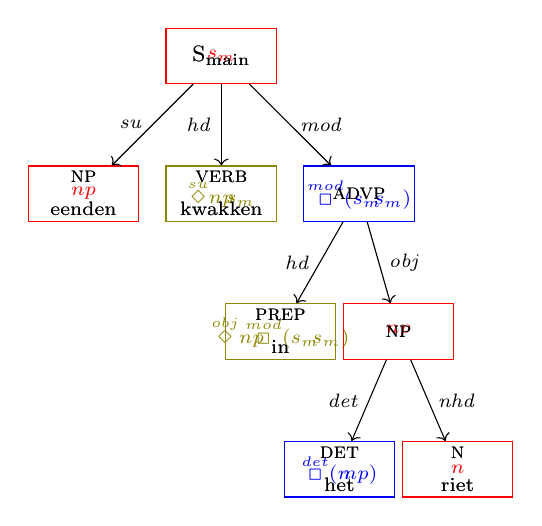
\begin{tikzpicture}[
	every text node part/.style={align=center},
	every node/.style={transform shape},
	block/.style={rectangle, inner sep=0pt, minimum width=40pt, minimum height=20pt},
	rblck/.style={rectangle, draw=red, inner sep=0pt, minimum width=40pt, minimum height=20pt},
	bblck/.style={rectangle, draw=blue, inner sep=0pt, minimum width=40pt, minimum height=20pt},
	oblck/.style={rectangle, draw=olive, inner sep=0pt, minimum width=40pt, minimum height=20pt}	
	]
	
	\alt<3->{
	\node[block] (smain) 	at (0, 0) 			{\type{s_m}{red}};}{
	\alt<2>{
	\node[rblck] (smain) 	at (0, 0) 			{\smain};}{
	\node[block] (smain) 	at (0, 0) 			{\smain};}}
	
	\alt<3->{
	\node[block] (eenden) 	at (-1.75, -1.75)		{\type{np}{red}};}{
	\alt<2>{
	\node[rblck] (eenden) 	at (-1.75, -1.75)		{\cat{np}\\ \W{eenden}};}{
	\node[block] (eenden) 	at (-1.75, -1.75)		{\cat{np}\\ \W{eenden}};}}

	\alt<7->{
	\node[block] (kwakken) 	at (0, -1.75) 		{\type{\overset{su}{\Diamond}np \li s_m}{olive}};}{
	\alt<6>{	
	\node[oblck] (kwakken) 	at (0, -1.75) 		{\cat{verb}\\ \W{kwakken}};}{
	\node[block] (kwakken) 	at (0, -1.75) 		{\cat{verb}\\ \W{kwakken}};}}
	
	
	\alt<5->{
	\node[block] (ihr)		at (1.75, -1.75) 		{\type{\overset{mod}{\Box}(s_m\li s_m)}{blue}};}{
	\alt<4>{
	\node[bblck] (ihr)		at (1.75, -1.75) 		{\cat{advp}};}{
	\node[block] (ihr)		at (1.75, -1.75) 		{\cat{advp}};}}
	
	\alt<7->{
	\node[block] (in)		at (0.75, -3.5) 		{\type{\overset{obj}{\Diamond}np\!\li\!\!\overset{mod}{\Box}(s_m\li s_m) }{olive}};}{
	\alt<6>{
	\node[oblck] (in)		at (0.75, -3.5) 		{\cat{prep}\\ \W{in}};}{
	\node[block] (in)		at (0.75, -3.5) 		{\cat{prep}\\ \W{in}};}}
	
	\alt<3->{
	\node[block] (hr)		at (2.25, -3.5) 		{\type{np}{red}};}{
	\alt<2>{
	\node[rblck] (hr)		at (2.25, -3.5) 		{\cat{np}};}{
	\node[block] (hr)		at (2.25, -3.5) 		{\cat{np}};}}
	
	\alt<5->{
	\node[block] (h)			at (1.5, -5.25) 		{\type{\overset{det}{\Box}(n\li np)}{blue}};}{
	\alt<4>{
	\node[bblck] (h)			at (1.5, -5.25) 		{\cat{det}\\ \W{het}};}{
	\node[block] (h)			at (1.5, -5.25) 		{\cat{det}\\ \W{het}};}}
	
	\alt<3->{
	\node[block] (r)			at (3, -5.25) 		{\type{n}{red}};}{
	\alt<2>{
	\node[rblck] (r)			at (3, -5.25) 		{\cat{n}\\ \W{riet}};}{
	\node[block] (r)			at (3, -5.25) 		{\cat{n}\\ \W{riet}};}}
	
	\draw (smain) 	edge[->]		node[left] 	{\etext{su}} 	(eenden);
	\draw (smain) 	edge[->]		node[left] 	{\etext{hd}} 	(kwakken);
	\draw (smain) 	edge[->]		node[right] {\etext{mod}} 	(ihr);
	
	\draw (ihr)	 	edge[->]		node[left] 	{\etext{hd}} 		(in);
	\draw (ihr)	 	edge[->]		node[right] {\etext{obj}} 		(hr);
	
	\draw(hr)		edge[->]		node[left] 	{\etext{det}}		(h);
	\draw(hr)		edge[->]		node[right] {\etext{nhd}}		(r);
	\end{tikzpicture}\vfill
	
	``eenden kwakken in het riet''
	\end{minipage}%
	\scriptsize
	\begin{minipage}{0.5\textwidth}
	while graph not fully typed, do:
	\begin{itemize}
		\visible<2->{
		\item assign \textcolor{red}{stand-alone nodes}	\\
				\quad no incoming adjunct or head edge\\
				\visible<3->{\quad \textbf{type} via the $\mathcal{A}$-map}}
		\visible<4->{
		\item assign \textcolor{blue}{adjuncts}\\
				\quad incoming adjunct edge\\
				\quad parent is typed\\
				\visible<5->{\quad \textbf{type}\\
				\quad if mod: boxed endofunctor of parent\\
				\quad else:from comp sibs to parent}}
		\visible<6->{
		\item assign \textcolor{olive}{heads} \\
				\quad incoming head edge\\
				\quad parent is typed\\
				\quad no untyped complement sibs\\
				\visible<7->{\quad \textbf{type} from comp sibs to parent}}
	\end{itemize}
	\vfill
	\end{minipage}
\end{frame}

\begin{frame}{Harder case: unbounded dependencies}
	\small
	\begin{minipage}{0.5\textwidth}
	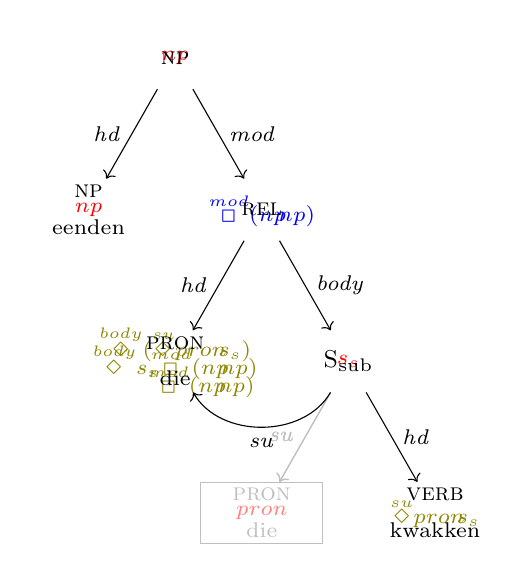
\begin{tikzpicture}[
	every text node part/.style={align=center},
	scale=1.1,
	every node/.style={transform shape},
	block/.style={rectangle, inner sep=0pt, minimum width=40pt, minimum height=20pt},
	rblck/.style={rectangle, draw=red, inner sep=0pt, minimum width=40pt, minimum height=20pt},
	bblck/.style={rectangle, draw=blue, inner sep=0pt, minimum width=40pt, minimum height=20pt},
	oblck/.style={rectangle, draw=olive, inner sep=0pt, minimum width=40pt, minimum height=20pt}	
	]
	
	\alt<3->{
	\node[block]		at (0, 0)			(root)		{\type{np}{red}};}{
	\node[block]		at (0, 0)			(root)		{\cat{np}};}
	
	\alt<3->{
	\node[block]		at (-1, -1.75)		(eenden)		{\type{np}{red}};}{
	\node[block]		at (-1, -1.75)		(eenden)		{\cat{np}\\ \W{eenden}};}
	
	\alt<3->{
	\node[block]		at (1, -1.75)		(dk)			{\type{\overset{mod}{\Box}(np \li np)}{blue}};}{
	\node[block]		at (1, -1.75)		(dk)			{\cat{rel}};}
	
	\alt<4->{
	\node[block]		at (0, -3.5)			(die)		
		{\type{\overset{body}{\Diamond}(\overset{su}{\Diamond}pron \li s_s)}{olive}\\
		\qquad \type{\li \overset{mod}{\Box}(np \li np)}{olive}};}{
	\alt<3->{
	\node[block]		at (0, -3.5)			(die)		{\type{\overset{body}{\Diamond}s_s \li \overset{mod}{\Box}(np \li np)}{olive}};}{
	\node[block]		at (0, -3.5)			(die)		{\cat{pron}\\ \W{die}};}}
	
	\alt<3->{
	\node[block]		at (2, -3.5)			(ssub)		{\type{s_{s}}{red}};}{
	\node[block]		at (2, -3.5)			(ssub)		{\ssub};}
	
	\alt<3->{
	\node[block]		at (3, -5.25)		(kwakken)	{\type{\overset{su}{\Diamond}pron \li s_s}{olive}};}{
	\node[block]		at (3, -5.25)		(kwakken)	{\cat{verb}\\ \W{kwakken}};}	
	
	\draw (root)		edge[->]		node[left] 	{\etext{hd}}		(eenden);	
	\draw (root)		edge[->]		node[right] {\etext{mod}}	(dk);
	\draw (dk)		edge[->]		node[left] 	{\etext{hd}}		(die);
	\draw (dk)		edge[->]		node[right] 	{\etext{body}}	(ssub);
	\draw (ssub)		edge[->]		node[right] 	{\etext{hd}}		(kwakken);	
	

	\alt<3->{
	\node[block]		at (1, -5.25)		(copy)	{\type{pron}{red!50}};
	\draw (ssub)		edge[->,draw=gray!50] node[left] {\textcolor{gray!50}{\etext{su}}}		(copy);
	}{
	\alt<2->{
	\node[block,draw=gray!50]		at (1, -5.25)		(copy)	{\textcolor{gray!50}{\cat{pron}}\\ \W{\textcolor{gray!50}{die}}};
	\draw (ssub)		edge[->,draw=gray!50] node[left] {\textcolor{gray!50}{\etext{su}}}		(copy);}{
	\draw (ssub)		edge[->, bend left=60] node[below] {\etext{su}}		(die);}}
	\end{tikzpicture}
	
	\begin{center}
		``eenden die kwakken''
	\end{center}	
	\end{minipage}%
	\begin{minipage}{0.5\textwidth}
	\scriptsize
	\begin{itemize}
	\visible<2->{
	\item 	detach non-local dependencies}
	\visible<3->{
	\item 	type trees as before}
	\visible<4->{
	\item	redact ghosts types from comp sibs}
	\end{itemize}
	\vfill
	\end{minipage}
\end{frame}

\begin{frame}{\alt<5>{ACG Flashback}{Hardest case: Ellipses}}
	\small
	
	\alt<5>{
	\begin{center}
		\vspace{5pt}
	\end{center}
	
	\footnotesize
	\begin{itemize}
		\item 	each conjunct represents a tuple of types \\
				$c = (t_1, t_2, \dots t_n) \equiv t_1 \lotimes t_2 \lotimes \dots \lotimes t_n$
		\item  encoded as the higher-order function $(c \li r)\li r$ and curried into 
		$(t_1 \li t_2 \li \dots \li t_n \li r)\li r$
	\end{itemize}
	}{
	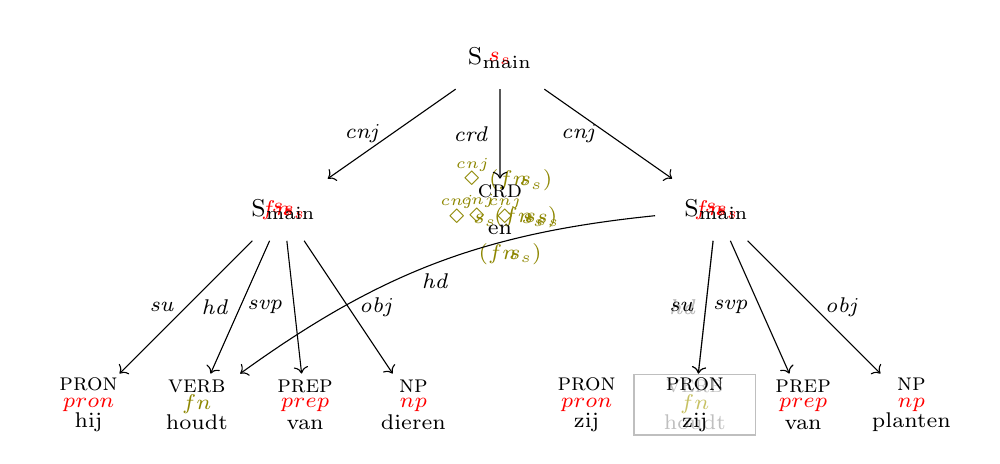
\begin{tikzpicture}[
	every text node part/.style={align=center},
	scale=1.1,
	every node/.style={transform shape},
	block/.style={rectangle, inner sep=0pt, minimum width=40pt, minimum height=20pt},
	rblck/.style={rectangle, draw=red, inner sep=0pt, minimum width=40pt, minimum height=20pt},
	bblck/.style={rectangle, draw=blue, inner sep=0pt, minimum width=40pt, minimum height=20pt},
	oblck/.style={rectangle, draw=olive, inner sep=0pt, minimum width=40pt, minimum height=20pt}	
	]
	\alt<3->{
	\node[block]			at (0, 0)			(root)		{\type{s_s}{red}};
	}{
	\node[block]			at (0, 0)			(root)		{\smain};}
	
	\alt<3->{
	\alt<4->{
	\node[block]			at (-2.5, -1.75)	(s1)				{\type{fn \li s_s}{red}};
	\node[block]			at (2.5, -1.75)		(s2)			{\type{fn \li s_s}{red}};
	}{
	\node[block]			at (-2.5, -1.75)	(s1)			{\type{s_s}{red}};
	\node[block]			at (2.5, -1.75)		(s2)			{\type{s_s}{red}};}
	\alt<6->{
	\node[block]			at (0, -1.75)		(en)			{
		\type{\overset{cnj}{\Diamond}(fn\li s_s)\li}{olive}\\
		~\type{\overset{cnj}{\Diamond}(fn\li s_s)\li}{olive}\\
		~~\type{(fn\li s_s)}{olive}};}{
	\node[block]			at (0, -1.75)		(en)			{\type{\overset{cnj}{\Diamond}s_s \li 
	\overset{cnj}{\Diamond}s_s \li s_s}{olive}};}}{
	\node[block]			at (-2.5, -1.75)	(s1)			{\smain};
	\node[block]			at (2.5, -1.75)		(s2)			{\smain};
	\node[block]			at (0, -1.75)		(en)			{\cat{crd}\\ \W{en}};}	
	
	\alt<3->{
	\node[block]			at (-4.75, -4)			(hij)		{\type{pron}{red}};
	\node[block]			at (-3.5, -4)			(houdt)		{\type{fn}{olive}};
	\node[block]			at (-2.25, -4)			(van)		{\type{prep}{red}};
	\node[block]			at (-1, -4)			(dieren)		{\type{np}{red}};}{
	\node[block]			at (-4.75, -4)			(hij)		{\cat{pron}\\ \W{hij}};
	\node[block]			at (-3.5, -4)			(houdt)		{\cat{verb}\\ \W{houdt}};
	\node[block]			at (-2.25, -4)			(van)		{\cat{prep}\\ \W{van}};
	\node[block]			at (-1, -4)			(dieren)		{\cat{np}\\ \W{dieren}};}

	\alt<3->{
	\node[block]			at (1, -4)			(zij)		{\type{pron}{red}};
	\node[block]			at (2.25, -4)		(houdt2)		{\type{fn}{olive!50}};
	\draw (s2)			edge[->,color=gray!50] node[left]	{\etext{\textcolor{gray!50}{hd}}} (houdt2);
	}{
	\alt<2->{
	\node[block]			at (1, -4)			(zij)		{\cat{pron}\\ \W{zij}};
	\node[block,draw=gray!50]			at (2.25, -4)			(houdt2)		{\cat{\textcolor{gray!50}{verb}}\\ \W{\textcolor{gray!50}{houdt}}};
	\draw (s2)			edge[->,color=gray!50] node[left]	{\etext{\textcolor{gray!50}{hd}}} (houdt2);}{
	\node[block]			at (2.25, -4)			(zij)		{\cat{pron}\\ \W{zij}};
	\draw (s2)			edge[->, bend right=15]			node[midway, below]			{\etext{hd}}			(houdt);	}}
	
	\alt<3->{
	\node[block]			at (3.5, -4)			(van2)			{\type{prep}{red}};
	\node[block]			at (4.75, -4)		(planten)		{\type{np}{red}};}{
	\node[block]			at (3.5, -4)			(van2)			{\cat{prep}\\ \W{van}};
	\node[block]			at (4.75, -4)		(planten)		{\cat{np}\\ \W{planten}};}

	\draw (root)			edge[->]			node[left]	{\etext{crd}}		(en);
	\draw (root)			edge[->]			node[left]	{\etext{cnj}}		(s1);
	\draw (root)			edge[->]			node[left]	{\etext{cnj}}		(s2);
	
	\draw (s1)			edge[->]			node[left]	{\etext{su}}			(hij);	
	\draw (s1)			edge[->]			node[left]	{\etext{hd}}			(houdt);	
	\draw (s1)			edge[->]			node[left]	{\etext{svp}}		(van);	
	\draw (s1)			edge[->]			node[right]	{\etext{obj}}		(dieren);	

	\draw (s2)			edge[->]			node[left]	{\etext{su}}			(zij);	
	\draw (s2)			edge[->]			node[left]	{\etext{svp}}			(van2);	
	\draw (s2)			edge[->]			node[right]	{\etext{obj}}		(planten);	
	\end{tikzpicture}
	\begin{center}
		``hij houdt van dieren en zij van planten''
	\end{center}
	
	\begin{minipage}{0.58\textwidth}
	\scriptsize
	\begin{itemize}
	\visible<2->{
	\item 	detach and type trees as usual}
	\visible<4->{
	\item 	redact missing types from \textbf{both} conjuncts}
	\visible<5->{
	\item update coord type \& attach copies at top level}
	\end{itemize}
	\end{minipage}%
	\begin{minipage}{0.42\textwidth}
	\scriptsize
	\begin{flushright}
		\visible<3->{
		$fn := \overset{svp}{\Diamond}prep \li \overset{obj}{\Diamond}{np}\li \overset{su}{\Diamond}pron \li s_s$}
	\end{flushright}
	\end{minipage}
	}
\end{frame}

\begin{frame}{Hardest case: Ellipses}
	\small
	
	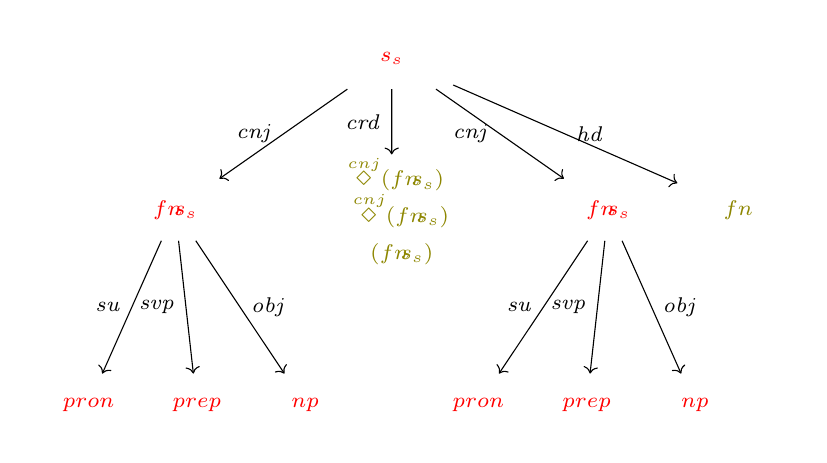
\begin{tikzpicture}[
	every text node part/.style={align=center},
	scale=1.1,
	every node/.style={transform shape},
	block/.style={rectangle, inner sep=0pt, minimum width=40pt, minimum height=20pt},
	rblck/.style={rectangle, draw=red, inner sep=0pt, minimum width=40pt, minimum height=20pt},
	bblck/.style={rectangle, draw=blue, inner sep=0pt, minimum width=40pt, minimum height=20pt},
	oblck/.style={rectangle, draw=olive, inner sep=0pt, minimum width=40pt, minimum height=20pt}	
	]
	\node[block]			at (0, 0)			(root)		{\type{s_s}{red}};
	\node[block, outer sep=0pt]			at (4, -1.75)		(houdt)		{\type{fn}{olive}};
		
	\node[block]			at (-2.5, -1.75)	(s1)				{\type{fn \li s_s}{red}};
	\node[block]			at (2.5, -1.75)		(s2)			{\type{fn \li s_s}{red}};
	\node[block]			at (0, -1.75)		(en)			{
		\type{\overset{cnj}{\Diamond}(fn\li s_s)\li}{olive}\\
		~\type{\overset{cnj}{\Diamond}(fn\li s_s)\li}{olive}\\
		~~\type{(fn\li s_s)}{olive}};
	
	\node[block]			at (-3.5, -4)			(hij)		{\type{pron}{red}};
	\node[block]			at (-2.25, -4)			(van)		{\type{prep}{red}};
	\node[block]			at (-1, -4)			(dieren)			{\type{np}{red}};
	\node[block]			at (1, -4)			(zij)			{\type{pron}{red}};

	\node[block]			at (2.25, -4)			(van2)		{\type{prep}{red}};
	\node[block]			at (3.5, -4)		(planten)			{\type{np}{red}};


	\draw (root)			edge[->]			node[left]	{\etext{crd}}		(en);
	\draw (root)			edge[->]			node[left]	{\etext{cnj}}		(s1);
	\draw (root)			edge[->]			node[left]	{\etext{cnj}}		(s2);
	
	\draw (s1)			edge[->]			node[left]	{\etext{su}}			(hij);	
	\draw (s1)			edge[->]			node[left]	{\etext{svp}}		(van);	
	\draw (s1)			edge[->]			node[right]	{\etext{obj}}		(dieren);	

	\draw (s2)			edge[->]			node[left]	{\etext{su}}			(zij);	
	\draw (s2)			edge[->]			node[left]	{\etext{svp}}		(van2);	
	\draw (s2)			edge[->]			node[right]	{\etext{obj}}		(planten);	
	\draw (root)			edge[->]			node[right]	{\etext{hd}}			(houdt);
	\end{tikzpicture}
	\begin{center}
		``hij houdt van dieren en zij van planten''
	\end{center}
	
	\begin{minipage}{0.58\textwidth}
	\scriptsize
	\begin{itemize}
	\item 	detach and type trees as usual
	\item 	redact missing types from \textbf{both} conjuncts
	\item update coord type \& attach copies at top level
	\end{itemize}
	\end{minipage}%
	\begin{minipage}{0.42\textwidth}
	\scriptsize
	\begin{flushright}
		$fn := \overset{svp}{\Diamond}prep \li \overset{obj}{\Diamond}{np}\li \overset{su}{\Diamond}pron \li s_s$
	\end{flushright}
	\end{minipage}
\end{frame}

\begin{frame}{A glimpse at a higher universe}
\small
	Second-order IL (system $F$ or polymorphic $\lambda$-calculus)
	
	\begin{align*}
		\infer[]{\Gamma \vdash \term{M\tau}: \sigma[\tau/ \alpha]}{\Gamma \vdash \term{M}: \forall \alpha.\sigma}
		&
		\qquad
		\textcolor{gray}{
		\infer[]{\Gamma \vdash \term{\Lambda \alpha.M}: \forall \alpha.\sigma}{\Gamma \vdash \term{M}: \sigma}}
	\end{align*}
	
	\pause
	In that universe, modifiers and coordinators are polymorphic types:
	\[
		\text{mod} := \term{\Lambda \alpha.w} :\forall \alpha.\Box^{mod}\left(\alpha \li \alpha\right)
	\]
	and
	\[
		\text{crd} := \term{\Lambda \alpha.w} : \forall \alpha.\Diamond^{cnj}\alpha \li \Diamond^{cnj}\alpha \li \alpha
	\]
\end{frame}

\begin{frame}{Coordinators as derived types}
	\small
	Elliptical coordinators can also be seen as a transformation of basic types.
	If $c = (t_1 \lotimes t_2 \lotimes \dots \lotimes t_N)$ the conjoined tuples,
	\begin{align*}
		crd = &c \li c \li c\\
		\overset{vr}{\rightarrow} & c\li c \li (c\li s) \li s\\
		\overset{ar^0}{\rightarrow} & \left( \left(c\li s\right) \li s \right) \li c \li (c\li s) \li s\\
		\overset{ar^1}{\rightarrow} & \left( \left(c\li s\right) \li s \right) \li \left( \left(c\li s\right) \li s \right) \li (c\li s) \li s\\
		\equiv &\left(\left( t_1 \li t_2 \li \dots \li t_n \li s \right) \li s \right) \li \\
		& \quad \left(\left( t_1 \li t_2 \li \dots \li t_n \li s \right) \li s \right) \li \\
		& \quad\quad \left( t_1 \li t_2 \li \dots \li t_n \li s \right) \li s
	\end{align*}
		\begin{align*}
			&\Diamond^{cnj}S_{main} \li \Diamond^{cnj}S_{main} \li S_{main}\\
			\overset{vr^*}{\rightarrow}&\Diamond^{cnj}S_{main} \li \Diamond^{cnj}S_{main} \li fn \li S_{main}\\
		\overset{ar^1}{\rightarrow}&\Diamond^{cnj}(fn \li S_{main}) \li \Diamond^{cnj}S_{main} \li fn \li S_{main}\\
		\overset{ar^2}{\rightarrow}&\Diamond^{cnj}(fn \li S_{main}) \li \Diamond^{cnj}(fn \li S_{main}) \li fn \li S_{main}
		\end{align*}
	\vfill
	\begin{itemize}
		\item \textbf{Value Raising}\\
			{\footnotesize
			From $f: \vec{A}\li B$ derive $\vec{A} \li (B\li D) \li D$
			}
		\item \textbf{Argument Raising}\\
			\begin{footnotesize}
			From $f: \vec{A}\li B \li \vec{C}\li D$ derive $\vec{A}\li ((B\li D)\li D) \li \vec{C} \li D$							\end{footnotesize}
	\end{itemize}
\end{frame}


\begin{frame}{From graphs to proofs}
	\centering
	\scriptsize
	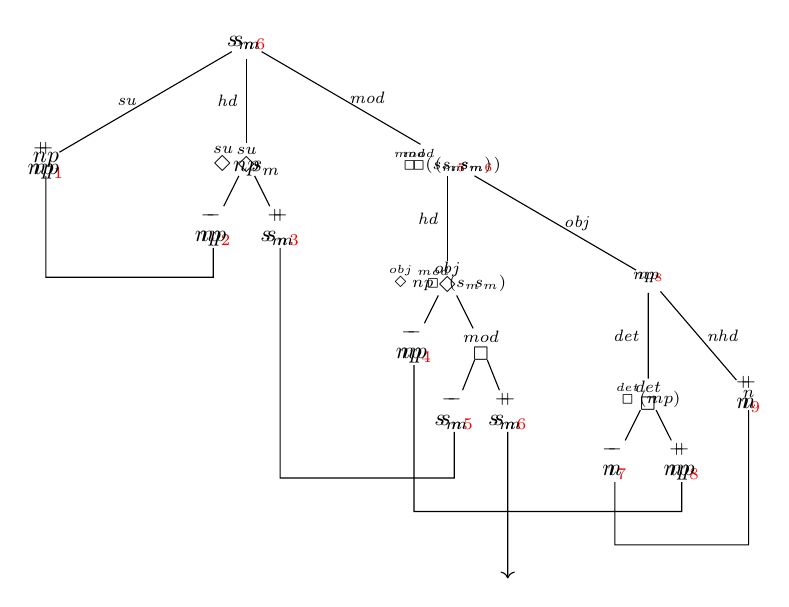
\begin{tikzpicture}[
	every text node part/.style={align=center},
	every node/.style={transform shape},
	scale=0.85,
	block/.style={rectangle, inner sep=0pt, minimum width=10pt, minimum height=13pt},
	level distance=30pt,
	every leaf node/.style={inner sep=0pt, inner xsep=0pt, outer sep=0pt,distance from root =150pt},
	sibling distance=0.5pt,
	grow=down
	]
	
	\alt<3->{
	 tree repr
	\alt<4->{
		\node[block] (r)			at (7.5, -5.25) 		{$\posat{n}\red{9}$};
		 atoms indexed
		\node[block]	(hn)			at (5.5, -6.25)		{$\negat{n}\red{7}$};
		\node[block]	(hnp)		at (6.5, -6.25)		{$\posat{np}\red{8}$};
		\node[block] (insm1)		at (3.1, -5.5)		{$\negat{s_m}\red{5}$};
		\node[block] (insm2)		at (3.9, -5.5)		{$\posat{s_m}\red{6}$};
		\node[block] (kwakkennp) at (-0.5, -2.75) 	{$\negat{np}\red{2}$};
		\node[block] (kwakkens) 	at (0.5, -2.75) 		{$\posat{s_m}\red{3}$};
		\node[block] (innp)		at (2.5, -4.5)		{$\negat{np}\red{4}$};
		\node[block] (eenden) 	at (-3, -1.75)		{$\posat{np}\red{1}$};
	}{
		\node[block] (r)			at (7.5, -5.25) 		{$\posat{n}$};
		\node[block]	(hn)			at (5.5, -6.25)		{$\negat{n}$};
		\node[block]	(hnp)		at (6.5, -6.25)		{$\posat{np}$};
		\node[block] (insm1)		at (3.1, -5.5)		{$\negat{s_m}$};
		\node[block] (insm2)		at (3.9, -5.5)		{$\posat{s_m}$};
		\node[block] (kwakkennp) at (-0.5, -2.75) 	{$\negat{np}$};
		\node[block] (kwakkens) 	at (0.5, -2.75) 		{$\posat{s_m}$};
		\node[block] (innp)		at (2.5, -4.5)		{$\negat{np}$};
		\node[block] (eenden) 	at (-3, -1.75)		{$\posat{np}$};}
		
	\node[block] (kwakkensu) at (0, -1.75) 		{$\overset{su}{\Diamond}$};
	\draw (kwakkensu) edge (kwakkennp);
	\draw (kwakkensu) edge (kwakkens);

	\node[block] (inobj)		at (3, -3.5)			{$\overset{obj}{\Diamond}$};
	\node[block] (inmod)		at (3.5, -4.5)		{$\overset{mod}{\Box}$};
	\draw (inobj)	edge (innp);
	\draw (inobj)	edge (inmod);
	\draw (inmod)	edge (insm1);
	\draw (inmod)	edge (insm2);
	\node[block]	(h)			at (6, -5.25)		{$\overset{det}{\Box}$};
	\draw (h) edge (hn);
	\draw (h) edge (hnp);
	}{
	 flat repr
	\node[block] (eenden) 	at (-3, -1.75)		{$np$};
	\node[block] (kwakken) 	at (0, -1.75) 		{${\overset{su}{\Diamond}}np\li {s_m}$};
	\node[block] (in)		at (3, -3.5) 		{\type{\overset{obj}{\Diamond}np\!\li\!\!\overset{mod}{\Box}({s_m}\li {s_m}) }{black}};
	\node[block] (h)			at (6, -5.25) 		{\type{\overset{det}{\Box}(n\li np)}{black}};
	\node[block] (r)			at (7.5, -5.25) 		{\type{n}{black}};}

	\alt<7->{	
	\node[block] (smain) 	at (0, 0) 			{$s_m\red{6}$};	
	\draw (kwakkens) -- (0.5, -6.5) -- (3.1, -6.5) -- (insm1);
	\draw (insm2)	edge[->] (3.9, -8);
	}{
	\node[block] (smain) 	at (0, 0) 			{$s_m$};	
	}
	
	\alt<6->{
	\node[block] (ihr)		at (3, -1.75) 		{\type{\overset{mod}{\Box}(s_m\red{5}\li s_m\red{6})}{black}};
	\draw (hnp) -- (6.5, -7) -- (2.5, -7) -- (innp);
	}{
	\node[block] (ihr)		at (3, -1.75) 		{\type{\overset{mod}{\Box}(s_m\li s_m)}{black}};}

	\alt<5->{
	\node[block] (hr)		at (6, -3.5) 		{\type{np\red{8}}{black}};
	\draw (hn) -- (5.5, -7.5) -- (7.5, -7.5) -- (r);
	\draw (eenden) -- (-3, -3.5) -- (-0.5, -3.5) -- (kwakkennp);
	}{	
	\node[block] (hr)		at (6, -3.5) 		{\type{np}{black}};}

	
	\draw (smain) 	edge[-]		node[left] 	{\etext{su}} 	(eenden);
	\draw (smain) 	edge[-]		node[left] 	{\etext{hd}} 	(kwakken);
	\draw (smain) 	edge[-]		node[right] {\etext{mod}} 	(ihr);
	
	\draw (ihr)	 	edge[-]		node[left] 	{\etext{hd}} 		(in);
	\draw (ihr)	 	edge[-]		node[right] {\etext{obj}} 		(hr);
	
	\draw(hr)		edge[-]		node[left] 	{\etext{det}}		(h);
	\draw(hr)		edge[-]		node[right] {\etext{nhd}}		(r);
	\end{tikzpicture}
	\vfill
	
	\visible<1>{given a typed graph:\\}
	\alt<2>{(1) convert types to binary trees and assign polarities}
	{\alt<3>{(2) assign identifying indices}{
	\alt<8>{the resulting structure is a \textit{proof net}
	\[
	\visible<6->{\blacktriangledown^{mod} \left(}
			\W{in} 
			\visible<2->{\vartriangle^{obj}\!\!
			\left( 
				\visible<4->{
				\blacktriangledown^{det}}
				\visible<3->{\W{het}}\
				\visible<5->{\W{riet}}
				}
			\right)
		\visible<6->{\right)}\ 
		\visible<7->{\left(\W{kwakken}}
		\visible<8->{\vartriangle^{su}\!\!\W{eenden}}
		\visible<7->{\right)}
	\]
	}{
	\alt<4->{(3) traverse upwards, identifying pos/neg atoms and propagating indices
	}}{}}}
	\visible<4-7>{
	\[
	\{2 \mapsto \alt<5->{1}{?}, 4 \mapsto \alt<6->{8}{?}, 5\mapsto \alt<7->{3}{?}, 7\mapsto \alt<5->{9}{?}\}
	\]
	}
\end{frame}

%
%\begin{frame}{From proofs to terms}
%	\centering
%	\scriptsize
%	\begin{tikzpicture}[
%	every text node part/.style={align=center},
%	every node/.style={transform shape},
%	scale=0.85,
%	block/.style={rectangle, inner sep=0pt, minimum width=10pt, minimum height=13pt},
%	level distance=30pt,
%	every leaf node/.style={inner sep=0pt, inner xsep=0pt, outer sep=0pt,distance from root =150pt},
%	sibling distance=0.5pt,
%	grow=down
%	]
%	
%	\node[block] (r)			at (7.5, -5.25) 		{$\posat{n}\red{9}$};
%	% atoms indexed
%	\node[block]	(hn)			at (5.5, -6.25)		{$\negat{n}\red{7}$};
%	\node[block]	(hnp)		at (6.5, -6.25)		{$\posat{np}\red{8}$};
%	\node[block] (insm1)		at (3.1, -5.5)		{$\negat{s_m}\red{5}$};
%	\node[block] (insm2)		at (3.9, -5.5)		{$\posat{s_m}\red{6}$};
%	\node[block] (kwakkennp) at (-0.5, -2.75) 	{$\negat{np}\red{2}$};
%	\node[block] (kwakkens) 	at (0.5, -2.75) 		{$\posat{s_m}\red{3}$};
%	\node[block] (innp)		at (2.5, -4.5)		{$\negat{np}\red{4}$};
%	\node[block] (eenden) 	at (-3, -1.75)		{$\posat{np}\red{1}$};
%
%		
%	\node[block] (kwakkensu) at (0, -1.75) 		{$\overset{su}{\Diamond}$};
%	\draw (kwakkensu) edge (kwakkennp);
%	\draw (kwakkensu) edge (kwakkens);
%
%	\node[block] (inobj)		at (3, -3.5)			{$\overset{obj}{\Diamond}$};
%	\node[block] (inmod)		at (3.5, -4.5)		{$\overset{mod}{\Box}$};
%	\draw (inobj)	edge (innp);
%	\draw (inobj)	edge (inmod);
%	\draw (inmod)	edge (insm1);
%	\draw (inmod)	edge (insm2);
%	\node[block]	(h)			at (6, -5.25)		{$\overset{det}{\Box}$};
%	\draw (h) edge (hn);
%	\draw (h) edge (hnp);
%	
%
%
%	\node[block] (smain) 	at (0, 0) 			{$s_m\red{6}$};	
%	\draw (kwakkens) -- (0.5, -6.5) -- (3.1, -6.5) -- (insm1);
%	\draw (insm2)	edge[->] (3.9, -8);
%		
%	\	\node[block] (ihr)		at (3, -1.75) 		{\type{\overset{mod}{\Box}(s_m\red{5}\li s_m\red{6})}{black}};
%	\draw (hnp) -- (6.5, -7) -- (2.5, -7) -- (innp);
%
%	\node[block] (hr)		at (6, -3.5) 		{\type{np\red{8}}{black}};
%	\draw (hn) -- (5.5, -7.5) -- (7.5, -7.5) -- (r);
%	\draw (eenden) -- (-3, -3.5) -- (-0.5, -3.5) -- (kwakkennp);
%	
%	
%	\draw (smain) 	edge[-]		node[left] 	{\etext{su}} 	(eenden);
%	\draw (smain) 	edge[-]		node[left] 	{\etext{hd}} 	(kwakken);
%	\draw (smain) 	edge[-]		node[right] {\etext{mod}} 	(ihr);
%	
%	\draw (ihr)	 	edge[-]		node[left] 	{\etext{hd}} 		(in);
%	\draw (ihr)	 	edge[-]		node[right] {\etext{obj}} 		(hr);
%	
%	\draw(hr)		edge[-]		node[left] 	{\etext{det}}		(h);
%	\draw(hr)		edge[-]		node[right] {\etext{nhd}}		(r);
%	\end{tikzpicture}
%	
%	\[
%		\visible<6->{\blacktriangledown^{mod} \left(}
%			\W{in} 
%			\visible<2->{\vartriangle^{obj}\!\!
%			\left( 
%				\visible<4->{
%				\blacktriangledown^{det}}
%				\visible<3->{\W{het}}\
%				\visible<5->{\W{riet}}
%				}
%			\right)
%		\visible<6->{\right)}\ 
%		\visible<7->{\left(\W{kwakken}}
%		\visible<8->{\vartriangle^{su}\!\!\W{eenden}}
%		\visible<7->{\right)}
%	\]
%\end{frame}

\begin{frame}{..continuing}
\small
The agenda:
\begin{itemize}
	\item[$\lambda$] \textcolor{gray}{Choosing the logic}
	\item[$\lambda$] \textcolor{gray}{Making a dataset: proofs and lexical type assignments}
	\item[$\lambda$] \alert{Learning the type assignment process}
	\item[$\lambda$] \alert{Navigating the proof space}
	\item[$\lambda$] \textcolor{gray}{Syntax-aware \& type-correct text representations}
\end{itemize}
\end{frame}

\begin{frame}{Lexical type ambiguity}
	\small
	
	\alt<3>{
	\begin{figure}
		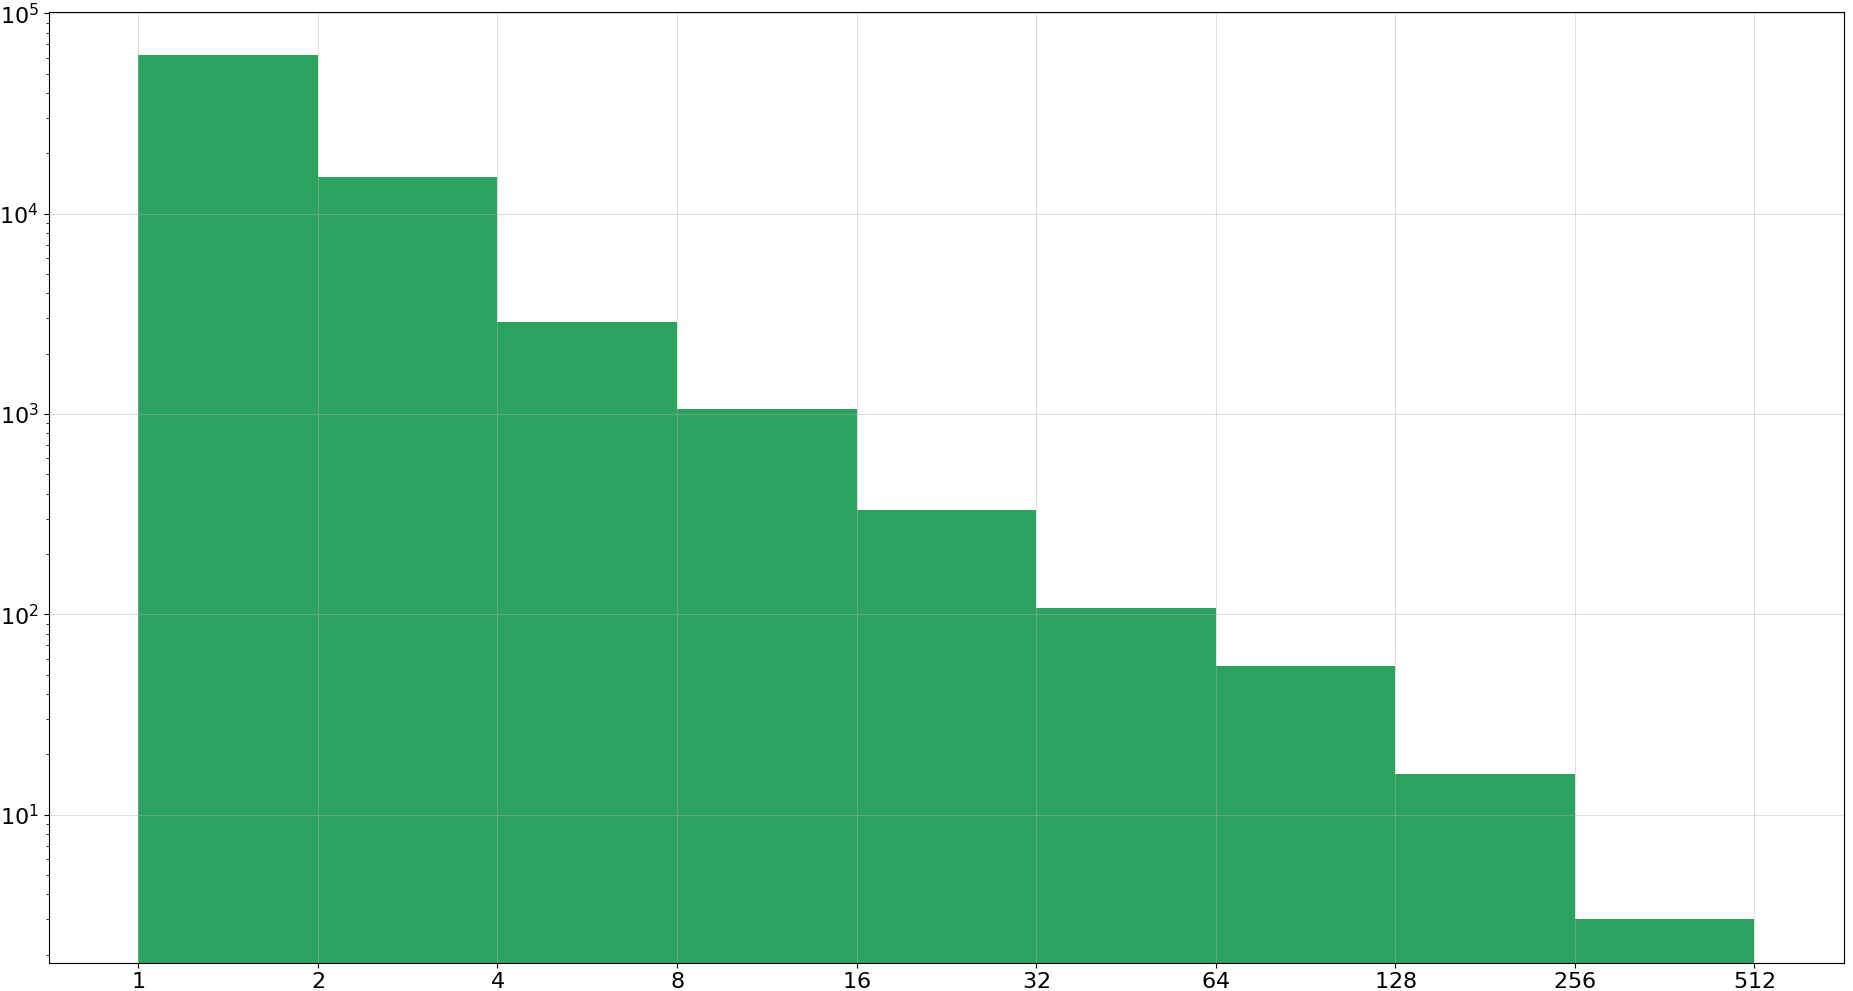
\includegraphics[width=0.99\textwidth]{oracle.png}
		\caption{\# types {\footnotesize(\textit{log2-transformed})} per word}
	\end{figure}
	}{
	\alt<2>{
		generally:
		\[
			w :: t_1 \& t_2 \& t_3 \& \dots \& t_n
		\]
		\vfill
			
		more refined grammar $\implies$ 
		\begin{itemize}
			\item[\frownie] harder lexical disambiguation (more $n$ per word)
			\item[\smiley]  easier parsing (\textit{if} one starts from correct type)
		\end{itemize}
	}{
	Type assignments are often \textit{ambiguous} and context-dependent:\vfill

	\begin{center}
	\begin{tabularx}{0.8\textwidth}{@{}rcl@{}}
	\multicolumn{3}{c}{\textbf{very realistic lexicon}}\\
	\toprule
	running :: 	& $\bx{mod}\left( np \li np \right)$ 					& \textit{running dog}\\
				& $inf$													& \textit{I like running}\\
	like		::	& $\dx{obj}np \li \dx{su}np \li s_m$					& \textit{ducks like seeds}\\
				& $\dx{obj}np \li \dx{su}pron \li s_m$					& \textit{I like ducks}\\
				& $\dx{obj}inf \li \dx{su}np \li s_m$					& \textit{ducks like swimming}\\
				& $\dx{obj}inf \li \dx{su}pron \li s_m$				& \textit{I like swimming}\\
				& $\dx{obj}np \li \bx{mod}\left( s_m \li s_m \right)$	& \textit{I swim like a duck}\\
				& \dots \\
	\end{tabularx}
	\end{center}
	}}
\end{frame}

\begin{frame}{Supertagging}
	\small
	
	\begin{block}{General idea}
		Given a sentence $w_1, w_2, \dots , w_n$\\
		\quad find the type sequence $t_1, t_2, \dots t_n$ that maximimizes
		\[
			p(t_1, t_2, \dots t_n | w_1, w_2, \dots w_n, \theta)
		\]
		where $\theta$ the trainable parameter space
	\end{block}
\end{frame}

\begin{frame}{Paleolithic ages}
	\small 
	\begin{block}{Indipendence Assumption}
	\[
		max(	p(t_1, t_2, \dots t_n | w_1, w_2, \dots w_n, \theta)) \approx \prod_{i=1}^{n} max(p(t_i, w_i, \theta))
	\]
	\end{block}

	Implemented as naive bayes/maximum entropy models, later using feed-forward networks on distributional vectors
	\begin{itemize}
		\item[\smiley] Beats hand-writing a lexicon
		\item[\frownie] Small (if any) context/receptive field
		\item[\frownie] No domain generalization 
		\item[\frownie] Severe sample sparsity when using windows
	\end{itemize}

\end{frame}

\begin{frame}{Discriminative approach}
	\small
	
	\begin{block}{Markov assumption}
		\begin{align*}
			& p(t_1, t_2, \dots t_n | w_1, w_2, \dots w_n, \theta) \\
			\approx &
			\prod_{i=1}^{n} p(t_i | w_1, w_2, \dots w_n, \theta)
		\end{align*}
	\end{block}
	
	Implemented as contextualized token classification using RNNs
	\begin{itemize}
		\item[\smiley] 			global context (lossy)
		\item[\smiley] 			domain generalization
		\item[\alert{\frownie}]	single answer
		\item[\alert{\frownie}]	sample sparsity
		\item[\alert{\frownie}]  no codomain generalization (closed world assumption)
	\end{itemize}
\end{frame}

\begin{frame}{Generative approach}
	\small
	
	\begin{block}{\st{Markov assumption}}
		\begin{align*}
			& p(t_1, t_2, \dots t_n | w_1, w_2, \dots w_n, \theta) \\
			\approx &
			\prod_{i=1}^{n} p(t_i | t_1, t_2, \dots, t_{i-1}, w_1, w_2, \dots w_n, \theta)
		\end{align*}
	\end{block}
	
	(could be) implemented as a transducer/seq2seq model
	\begin{itemize}
		\item[\smiley]			global context (lossless)
		\item[\smiley]			many answers
		\item[\alert{\frownie}]	sample sparsity 
		\item[\alert{\frownie}]	no codomain generalization
	\end{itemize}
\end{frame}

\begin{frame}{Generative approach: one more step}
	\small
	The type syntax: 
	\[
		cod(\mathcal{L}) := A \ | \ \dx{d} T \li T' \ | \ \bx{d}\left( T \li T' \right)
	\]
	corresponds to a \alert{simple cfg} (in prefix notation) with meta-rules:
		\begin{align*}
			S & \to A 				& & \forall A \in \mathcal{A}\\
			S & \to \dx{d} S \ S	& & \forall d \in \mathrm{comps} \\
			S & \to \bx{d} S \ S 	& & 	\forall d \in \mathrm{adjns}
		\end{align*}
	i.e. each type $t_i$ can be written as a sequence of primitive symbols $\vec{\sigma}$
	
	\pause
	\begin{align*}
			& p(t_1, t_2, \dots t_n | w_1, w_2, \dots w_n, \theta) \\
			\approx &
			\prod_{i=1}^{n} p(\sigma_i | \sigma_1, \sigma_2, \dots, \sigma_{i-1}, w_1, w_2, \dots w_n, \theta)
	\end{align*}
	
	\begin{itemize}
		\item[\smiley]			each type contains many subtypes (less sparsity)
		\item[\smiley]			any valid types can be inductively constructed (open codomain)
	\end{itemize}
\end{frame}

\begin{frame}{Supertagging today}
	\smaller
	\begin{itemize}
		\item[?] types are \textbf{trees} -- but tree transduction requires trees decoded in isolation
		\pause
		\item[?] longer sequence length $\implies$ memory and time cost, degraded beam search
		\pause
		\item[?] harder to train: the system has to learn a grammar within the grammar
		\pause
		\item[?] left-right decoding does not make use of \textit{easy} types first
		\pause
		\item[?] logical constraints are not easy to integrate with neural decoding
		\pause
		\item[!] new possibilities for parsing and meaning representation
	\end{itemize}
	
\end{frame}

\begin{frame}{Proof Ambiguity}
	\small
	The type system (being non-directional) permits too many parses:
	\vfill
	
	\begin{minipage}{0.5\textwidth}
	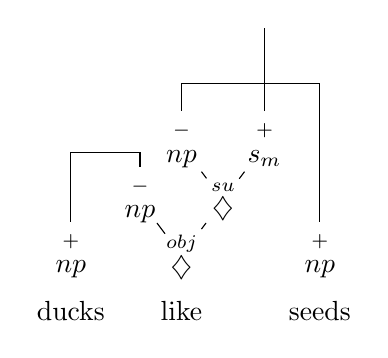
\begin{tikzpicture}[
	all node/.style={outer sep=0pt}
	]
		\node		(ducks)			at	(0,0)			{ducks};
		\node		(ducksnp)		at	(0,2em)			{$\posat{np}$};
		
		\node		(like)			at	(4em,0)			{like};
		\node		(likeobj)		at	(4em,2em)		{$\dx{obj}$};
		\node		(likenp1)		at 	(2.5em, 4em)		{$\negat{np}$};
		\node		(likesu)			at 	(5.5em, 4em)		{$\dx{su}$};
		\node		(likenp2)		at 	(4em, 6em)		{$\negat{np}$};
		\node		(likes)			at 	(7em, 6em)		{$\posat{s_m}$};
		\draw (likeobj) 	-- (likenp1);
		\draw (likeobj)	-- (likesu);
		\draw (likesu) 	-- (likenp2);
		\draw (likesu) 	-- (likes);
		\draw (likes)	-- ($(likes.north) + (0,3em)$);
		
		\node		(seeds)			at 	(9em, 0em)		{seeds};
		\node		(seedsnp)			at 	(9em, 2em)		{$\posat{np}$};
		
		\draw (ducksnp) -- ($(ducksnp.north) + (0,2.5em)$) -| ($(likenp1.north)$);
		\draw (seedsnp) -- ($(seedsnp.north) + (0,5em)$) -| ($(likenp2.north)$);
	\end{tikzpicture}	
	\centering
	\footnotesize
	\[
		\term{like\ (ducks)^{obj}\ (seeds)^{su}}
	\]
	\end{minipage}%
	\begin{minipage}{0.5\textwidth}
	\hfill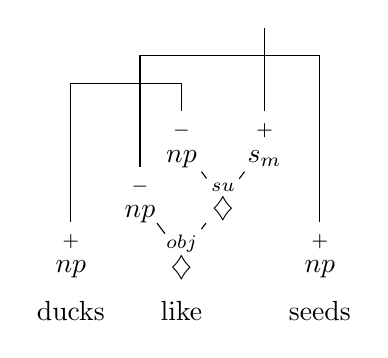
\begin{tikzpicture}
		\node		(ducks)			at	(0,0)			{ducks};
		\node		(ducksnp)		at	(0,2em)			{$\posat{np}$};
		
		\node		(like)			at	(4em,0)			{like};
		\node		(likeobj)		at	(4em,2em)		{$\dx{obj}$};
		\node		(likenp1)		at 	(2.5em, 4em)		{$\negat{np}$};
		\node		(likesu)			at 	(5.5em, 4em)		{$\dx{su}$};
		\node		(likenp2)		at 	(4em, 6em)		{$\negat{np}$};
		\node		(likes)			at 	(7em, 6em)		{$\posat{s_m}$};
		\draw (likeobj) 	-- (likenp1);
		\draw (likeobj)	-- (likesu);
		\draw (likesu) 	-- (likenp2);
		\draw (likesu) 	-- (likes);
		\draw (likes)	-- ($(likes.north) + (0,3em)$);
		
		\node		(seeds)			at 	(9em, 0em)		{seeds};
		\node		(seedsnp)		at 	(9em, 2em)		{$\posat{np}$};
		
		\draw (ducksnp) -- ($(ducksnp.north) + (0,5em)$) -| ($(likenp2.north)$);
		\draw (seedsnp) -- ($(seedsnp.north) + (0,6em)$) -| ($(likenp1.north)$);
	\end{tikzpicture}
	\centering
	\footnotesize
	\[
		\term{like\ (seeds)^{obj}\ (ducks)^{su}}
	\]
	\end{minipage}
	\vfill
	
	\pause
	\centering
	How can we select the correct one?
\end{frame}

\begin{frame}{Neural Proof Nets}
% pnet and tables
\scriptsize
\begin{center}
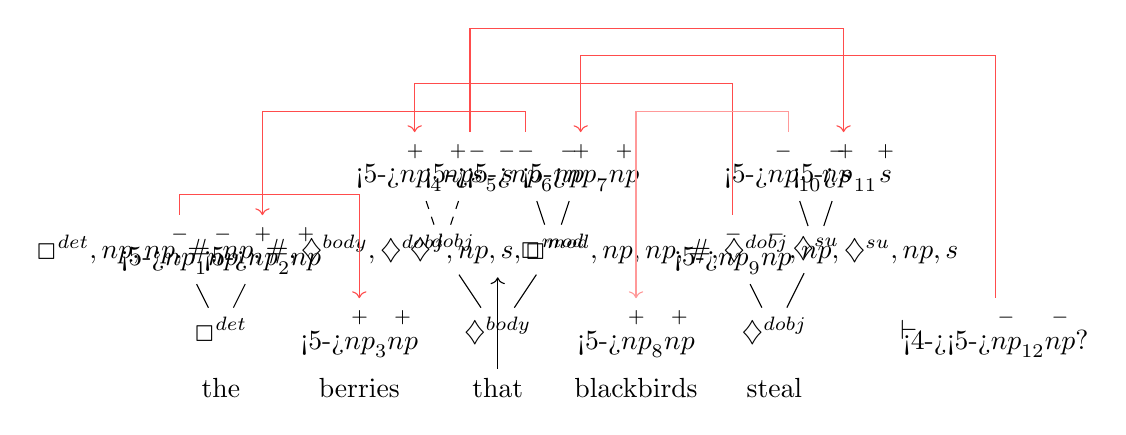
\begin{tikzpicture}
	% words
	\node (the)		at 	(0em, 0em)	{the};
	\node (berries)	at 	(5em, 0em)	{berries};
	\node (that)		at 	(10em, 0em)	{that};
	\node (birds) 	at 	(15em, 0em) 	{blackbirds};
	\node (steal)	at	(20em, 0em)	{steal};
	
	\visible<2-2>{
	\draw[->] (that) -- ($(10em, 4em)$);
	\node (test) 	at 	(10em, 5em) {
	$\Box^{det}, np, np, \#, np, \#, \diamondsuit^{body}, \diamondsuit^{dobj}, np, s, \Box^{mod}, np, np, \#, \diamondsuit^{dobj}, np, \diamondsuit^{su}, np, s$
	};
	}
	\visible<3->{
	% undecorated trees
	\node (thedet)		at	(0em, 2em)		{$\Box^{det}\proofspace$};
	\node (thenp1)		at	(-1.5em, 5em)	
		{\alt<5->{$\negat{np}_1$}{$\negat{np}$}};
	\node (thenp2)		at	(1.5em, 5em)		
		{\alt<5->{$\posat{np}_2$}{$\posat{np}$}};
	\node (berriesnp)	at 	(5em, 2em)		
		{\alt<5->{$\posat{np}_3$}{$\posat{np}$}};
	\node (thatbody)		at	(10em, 2em)		{$\diamondsuit^{body}\proofspace$};
	\node (thatobj)		at	(8em, 5em)		{$\diamondsuit^{dobj}\proofspace$};
	\node (thatobjnp)	at	(7em, 8em)		
		{\alt<5->{$\posat{np}_4$}{$\posat{np}$}};
	\node (thats)		at	(9em, 8em)		
		{\alt<5->{$\negat{s}_5$}{$\negat{s}$}};
	\node (thatmod)		at	(12em, 5em)		{$\Box^{mod}\proofspace$};
	\node (thatmodnp1)	at	(11em, 8em)		
		{\alt<5->{$\negat{np}_6$}{$\negat{np}$}};
	\node (thatmodnp2)	at	(13em, 8em)		
		{\alt<5->{$\posat{np}_7$}{$\posat{np}$}};
	\node (birdsnp)		at	(15em, 2em)		
		{\alt<5->{$\posat{np}_8$}{$\posat{np}$}};
	\node (stealobj)		at	(20em, 2em)		{$\diamondsuit^{dobj}\proofspace$};
	\node (stealobjnp)	at	(18.5em, 5em)	
		{\alt<5->{$\negat{np}_9$}{$\negat{np}$}};
	\node (stealsu)		at	(21.5em, 5em)	{$\diamondsuit^{su}\proofspace$};
	\node (stealsunp)	at  (20.5em, 8em)	
		{\alt<5->{$\negat{np}_{10}$}{$\negat{np}$}};
	\node (steals)		at 	(22.5em, 8em)	
		{\alt<5->{$\posat{s}_{11}$}{$\posat{s}$}};
	\node (vdash)		at 	(25em, 2em)		{$\vdash\proofspace$};
	\node (finalnp)		at 	(28em, 2em)		
		{\alt<4->{\alt<5->{$\negat{np}_{12}$}{$\negat{np}$}}{$?$}};
	
	% internal links
	\draw (thedet)   -- (thenp1);
	\draw (thedet)   -- (thenp2);
	\draw (stealobj) -- (stealobjnp);
	\draw (stealobj) -- (stealsu);
	\draw (stealsu)  -- (stealsunp);
	\draw (stealsu)  -- (steals);
	\draw (thatbody) -- (thatobj);
	\draw (thatobj)   edge[dashed] (thatobjnp);
	\draw (thatobj)   edge[dashed] (thats);
	\draw (thatmod)  -- (thatmodnp1);
	\draw (thatmod)  -- (thatmodnp2);
	\draw (thatbody) -- (thatmod);
	
	% axiom links
	\visible<8->{
	\draw[<-, red!70] (berriesnp) -- ($(berriesnp) + (0em, 5em)$) -| (thenp1);
	\draw[<-, red!70] (thenp2) -- ($(thenp2) + (0em, 5em)$) -| (thatmodnp1);
	\draw[<-, red!70] (thatobjnp) -- ($(thatobjnp) + (0em,3em)$) -| (stealobjnp);
	\draw[->, red!70] (thats) -- ($(thats) + (0em, 5em)$) -| (steals);
	\draw[<-, red!70] (thatmodnp2) -- ($(thatmodnp2) + (0em, 4em)$) -| (finalnp);
	\draw[<-, red!40] (birdsnp) -- ($(birdsnp) + (0em, 8em)$) -| (stealsunp);
	}
	}
\end{tikzpicture}
\end{center}	
\vfill

\begin{minipage}[c]{0.75\textwidth}
\alt<2->{
\alt<3->
{
\alt<4->
{
\alt<5->
{
\alt<6->
{
\alt<7->
{7. train against ground-truth axiom links}
{6. discretize result with \textrm{Sinkhorn}}
}
{5. fill table with pair-wise agreement scores}
}
{4. index pos/neg occurrences and arrange in a table}
}
{3. find conclusion as the singleton $\mathcal{A}^+ - \mathcal{A}^-$}
}
{2. parse types to trees and assign polarity information}
}
{
1. pass the sentence through the supertagger
}
\end{minipage}%
\begin{minipage}[c]{0.25\textwidth}
\visible<5->{
		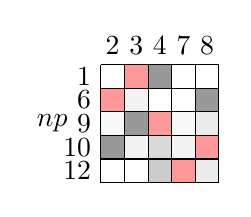
\begin{tikzpicture}[scale=.3]
		% matches
		\visible<6>{
		\fill[gray!60] (1, 4) rectangle +(1,1);
		\fill[gray!10] (1, 1) rectangle +(1,1);
		\fill[gray!20] (1, 2) rectangle +(1,1);
		\fill[gray!10] (1, 3) rectangle +(1,1);
		\fill[gray!80] (0, 3) rectangle +(1,1);
		\fill[gray!5] (0, 2) rectangle +(1,1);
		\fill[gray!5] (0, 1) rectangle +(1,1);
		\fill[gray!40] (2, 2) rectangle +(1,1);
		\fill[gray!30] (2, 1) rectangle +(1,1);
		\fill[gray!40] (2, 0) rectangle +(1,1);
		\fill[gray!10] (2, 4) rectangle +(1,1);
		\fill[gray!50] (4, 1) rectangle +(1,1);
		\fill[gray!15] (4, 2) rectangle +(1,1);
		\fill[gray!15] (4, 0) rectangle +(1,1);
		\fill[gray!20] (4, 3) rectangle +(1,1);
		\fill[gray!90] (3, 0) rectangle +(1,1);
		\fill[gray!10] (3, 1) rectangle +(1,1);
		\fill[gray!5] (3, 2) rectangle +(1,1);
		\fill[gray!5] (3, 0) rectangle +(1,1);
		}
		\visible<7->{
		\fill[black!40] (1, 2) rectangle +(1,1);
		\fill[black!40] (0, 1) rectangle +(1,1);
		\fill[black!40] (2, 4) rectangle +(1,1);
		\fill[black!40] (4, 3) rectangle +(1,1);
		\fill[black!40] (3, 0) rectangle +(1,1);
		}
		\visible<8->{
		\fill[red!40] (1, 4) rectangle +(1,1);
		\fill[red!40] (0, 3) rectangle +(1,1);
		\fill[red!40] (2, 2) rectangle +(1,1);
		\fill[red!40] (4, 1) rectangle +(1,1);
		\fill[red!40] (3, 0) rectangle +(1,1);
		}
		\node [above] at (0.5, 5)	{2};
		\node [above] at (1.5, 5)	{3};
		\node [above] at (2.5, 5)	{4};
		\node [above] at (3.5, 5)	{7};
		\node [above] at (4.5, 5)	{8}; 
		\node [left] at (0, 4.5)		{1};
		\node [left] at (0, 3.5)		{6};
		\node [left] at (0, 2.5)		{9};
		\node [left] at (0, 1.5)		{10};    
	    \node [left] at (0,0.5) 		{12};
	    \node [left] at (-1,2.5)	 	{$np$};
	    \draw (0,0) grid (5,5);
	    \end{tikzpicture}
}
\end{minipage}
\end{frame}
	
\begin{frame}{The future}

\smaller
\begin{itemize}
	\item[$\lambda$] \textcolor{gray}{Choosing the logic}
	\item[$\lambda$] \textcolor{gray}{Making a dataset: proofs and lexical type assignments}
	\item[$\lambda$] \textcolor{gray}{Learning the type assignment process}
	\item[$\lambda$] \textcolor{gray}{Navigating the proof space}
	\item[$\lambda$] \alert{Syntax-aware \& type-correct text representations}\\
	\pause
	{\smaller
	\begin{itemize}
	 	 \item[-] meaning representation from proofs: graph traversal/encoding
	 	 \item[-] types as recipes/functions on word embeddings, pure interpretations of the system
	 	 \item[-] \dots
	 	 \item[-] {[your project/internship/thesis idea here]}
	\end{itemize}
	}
	\vfill
	
\flushright	diy: \url{github.com/konstantinosKokos/neural-proof-nets}
\end{itemize}\end{frame}


\end{document}
